\documentclass[11pt,a4paper,oneside]{report}

% ------------------------------------------------------------------------------
% Page Layout and Geometry (~2.5 cm margins)
% ------------------------------------------------------------------------------
\usepackage[a4paper, top=2.5cm, bottom=2.5cm, left=2.5cm, right=2.5cm]{geometry}

% ------------------------------------------------------------------------------
% Typography & Mathematics Fonts
% ------------------------------------------------------------------------------
\usepackage{amsmath, amssymb, amsthm}
\usepackage{mathptmx}
\usepackage{setspace}
\onehalfspacing

% ------------------------------------------------------------------------------
% Academic Color Palette (Professional Navy / Blue)
% ------------------------------------------------------------------------------
\usepackage{xcolor}
\definecolor{primaryblue}{RGB}{0, 45, 98}
\definecolor{secondarynavy}{RGB}{24, 76, 120}
\definecolor{darkgray}{RGB}{50, 50, 50}
\definecolor{lightgray}{RGB}{245, 245, 245}
\definecolor{codebackground}{RGB}{248, 249, 250}
\definecolor{codegreen}{RGB}{34, 139, 34}
\definecolor{codegray}{RGB}{128, 128, 128}

% ------------------------------------------------------------------------------
% Graphics, Tables & Floats
% ------------------------------------------------------------------------------
\usepackage{graphicx}
\graphicspath{{figures/}{latex/figures/}{./}}
\usepackage{booktabs}
\usepackage{caption}
\usepackage{subcaption}
\usepackage{float}

% ------------------------------------------------------------------------------
% TikZ Vector Diagram Support
% ------------------------------------------------------------------------------
\usepackage{tikz}
\usetikzlibrary{shapes.geometric, arrows.meta, positioning}
\tikzset{
    startstop/.style = {rectangle, rounded corners, minimum width=2.4cm, minimum height=0.7cm, text centered, draw=darkgray, fill=primaryblue!10, font=\small\bfseries},
    process/.style   = {rectangle, minimum width=2.6cm, minimum height=0.7cm, text centered, draw=darkgray, fill=secondarynavy!10, font=\small},
    decision/.style  = {diamond, minimum width=2.6cm, minimum height=0.8cm, text centered, draw=darkgray, fill=codebackground, aspect=2, font=\small},
    arrow/.style     = {thick, ->, >=stealth, color=darkgray}
}

% ------------------------------------------------------------------------------
% Running Headers & Footers
% ------------------------------------------------------------------------------
\usepackage{fancyhdr}
\pagestyle{fancy}
\fancyhf{}
\fancyhead[L]{\small\color{darkgray}Algorithm Explorer: Analytical \& Empirical Study}
\fancyhead[R]{\small\color{darkgray}\nouppercase{\leftmark}}
\fancyfoot[C]{\thepage}
\renewcommand{\headrulewidth}{0.4pt}
\renewcommand{\footrulewidth}{0.0pt}

% ------------------------------------------------------------------------------
% Listings for Python Code
% ------------------------------------------------------------------------------
\usepackage{listings}
\lstset{
    language=Python,
    backgroundcolor=\color{codebackground},
    basicstyle=\ttfamily\footnotesize\color{black},
    keywordstyle=\bfseries\color{primaryblue},
    stringstyle=\color{codegreen},
    commentstyle=\itshape\color{codegray},
    numbers=left,
    numberstyle=\tiny\color{codegray},
    stepnumber=1,
    numbersep=8pt,
    tabsize=4,
    showspaces=false,
    showstringspaces=false,
    breaklines=true,
    breakatwhitespace=true,
    frame=single,
    rulecolor=\color{lightgray},
    captionpos=b
}

% ------------------------------------------------------------------------------
% Theorems & Definitions
% ------------------------------------------------------------------------------
\theoremstyle{definition}
\newtheorem{definition}{Definition}[chapter]
\newtheorem{theorem}{Theorem}[chapter]
\newtheorem{example}{Example}[chapter]

% ------------------------------------------------------------------------------
% Chapter & Section Heading Formatting
% ------------------------------------------------------------------------------
\usepackage{titlesec}
\titleformat{\chapter}[hang]{\Huge\bfseries\color{primaryblue}}{\thechapter}{1em}{}
\titleformat{\section}{\Large\bfseries\color{secondarynavy}}{\thesection}{1em}{}
\titleformat{\subsection}{\large\bfseries\color{darkgray}}{\thesubsection}{1em}{}

% ------------------------------------------------------------------------------
% Hyperlinks & PDF Bookmarks
% ------------------------------------------------------------------------------
\usepackage[
    colorlinks=true,
    linkcolor=primaryblue,
    citecolor=secondarynavy,
    urlcolor=primaryblue,
    bookmarksnumbered=true,
    pdfstartview=FitH
]{hyperref}

% Metadata Constants
\newcommand{\DocTitle}{Algorithm Explorer: An Analytical and Empirical Study of Algorithms, Growth of Functions and Computational Complexity}
\newcommand{\DocSubtitle}{Algorithm Assignment Of Discrete Mathematics}
\newcommand{\DocAuthor}{Patel Arpit Dasharathbhai}
\newcommand{\DocRollNumber}{202612120}
\newcommand{\DocCourse}{MSc (Information Technology)}
\newcommand{\DocCourseCode}{MSc-IT-DM-2026}
\newcommand{\DocFaculty}{\href{https://algorithm-explorer.glitchhunter69.workers.dev/}{\texttt{https://algorithm-explorer.glitchhunter69.workers.dev/}}}
\newcommand{\DocUniversity}{LIVE : Algorithm Explorer}
\newcommand{\DocAcademicYear}{2026--2027}
\newcommand{\DocDate}{\today}

\begin{document}

% ==============================================================================
% COVER PAGE
% ==============================================================================
\begin{titlepage}
    \centering
    \vspace*{1.0cm}
    
    {\scshape\Large \DocUniversity \par}
    \vspace{0.3cm}
    {\scshape\large \DocFaculty \par}
    \vspace{0.3cm}
    {\large \DocCourse\ (\DocCourseCode) \par}
    
    \vspace{1.5cm}
    \rule{\linewidth}{1.2pt}\\[0.4cm]
    {\huge\bfseries\color{primaryblue} \DocTitle \par}
    \vspace{0.3cm}
    {\large\itshape \DocSubtitle \par}
    \rule{\linewidth}{1.2pt}
    
    \vspace{1.8cm}
    
    \begin{minipage}{0.48\textwidth}
        \begin{flushleft} \large
            \emph{Prepared by:}\\
            \textbf{\DocAuthor}\\
            Student ID: \texttt{\DocRollNumber}
        \end{flushleft}
    \end{minipage}
    \hfill
    \begin{minipage}{0.48\textwidth}
        \begin{flushright} \large
            \emph{Academic Subject:}\\
            \textbf{Discrete Mathematics \- SC612}\\
            Primary Reference: Rosen Ch.~3
        \end{flushright}
    \end{minipage}
    
    \vfill
    
    {\large Academic Session: \DocAcademicYear \par}
    {\large Date of Submission: \DocDate \par}
\end{titlepage}

% ==============================================================================
% FRONT MATTER: ROMAN NUMBERING
% ==============================================================================
\pagenumbering{roman}
\setcounter{page}{2}

% ABSTRACT
\begin{abstract}
This analytical monograph presents a rigorous, curriculum-aligned academic examination of fundamental algorithmic principles, the mathematical growth of functions, and computational complexity as articulated in Chapter~3 of Kenneth~H. Rosen's \emph{Discrete Mathematics and Its Applications} (8th Edition). Grounded in the faculty's analytical assignment specifications, this study investigates four required discrete mathematical topics: (1) the definition, characteristics, and multi-paradigm representations of algorithms; (2) systematic algorithmic typology, contrasting problem categories with design strategies; (3) asymptotic growth hierarchies ($1 \prec \log n \prec n \prec n \log n \prec n^2 \prec 2^n \prec n!$), supported by closed-form evaluations and numerical tables; and (4) formal computational complexity ($\mathcal{O}, \Omega, \Theta$) spanning best-, worst-, and average-case performance.

To bridge theoretical proofs with empirical validation, four canonical algorithms are subjected to exhaustive practical study: Linear Search, Binary Search, Bubble Sort (Rosen's fixed-pass formulation), and Insertion Sort. Using a verified Python 3.14.7 benchmarking testbed with hardware-calibrated nanosecond telemetry over $k = 30$ independent replications across scales up to $n = 100\,000$, we contrast exact analytical operation-count formulas with empirical counts (yielding a verified 0.00\% discrepancy) and wall-clock execution times. All nine validated experimental figures and execution outputs generated through our Jupyter Research Notebook are integrated into this monograph. Additionally, an interactive standalone HTML5 web dashboard is presented to support visual, real-time algorithmic experimentation.
\end{abstract}

% \vspace{0.5cm}
% \noindent\textbf{Keywords:} Discrete Mathematics, Kenneth H. Rosen, Algorithm Analysis, Growth of Functions, Asymptotic Notations, Time Complexity, Linear Search, Binary Search, Bubble Sort, Insertion Sort, Inversion Equivalence.

\newpage
\tableofcontents
\newpage
\listoffigures
\vspace{0.5cm}
\listoftables

\newpage
% ==============================================================================
% MAIN MATTER: ARABIC NUMBERING
% ==============================================================================
\pagenumbering{arabic}
\setcounter{page}{1}

\chapter{Introduction}
\label{chap:introduction}

\section{Context of Algorithms in Discrete Mathematics}
In discrete mathematics and theoretical computer science, algorithms constitute the foundational mechanisms by which computational problems are formally analyzed and solved. Kenneth~H. Rosen, in Chapter~3 of \emph{Discrete Mathematics and Its Applications} (8th Edition)~\cite{Rosen2019}, establishes that studying algorithms is not merely an exercise in software programming; rather, it is a mathematical discipline dedicated to demonstrating correctness, proving termination, and characterizing the computational resources required by deterministic procedures.

\section{Purpose and Scope of Algorithm Analysis}
The primary objective of algorithmic analysis is to determine how resource requirements---principally temporal duration (time complexity) and memory consumption (space complexity)---scale as the input size $n$ approaches infinity. By abstracting computational cost away from ephemeral platform parameters (such as CPU clock speed, compiler optimizations, and memory architecture), discrete mathematical analysis provides durable, invariant measures of efficiency.

\section{Assignment Objectives and Deliverables}
In strict adherence to the faculty's handwritten assignment instructions, this analytical note addresses the four mandatory academic topics:
\begin{enumerate}
    \item \textbf{What is an Algorithm?}: Formal definition, essential characteristics, and representation paradigms.
    \item \textbf{Types of Algorithms}: Classification by problem type and design paradigm, introducing our four core study algorithms.
    \item \textbf{The Growth of Functions}: Mathematical formulation of growth rates, the canonical hierarchy, and numerical evaluations.
    \item \textbf{Complexity of Algorithms}: Asymptotic notations ($\mathcal{O}, \Omega, \Theta$), case analysis, and practical study of four algorithms.
\end{enumerate}

The study unifies three submission deliverables: (1) this comprehensive analytical report, (2) the interactive, pre-executed Jupyter Research Notebook (\texttt{notebooks/algorithm\_explorer.ipynb}), and (3) the optional interactive HTML5 algorithm visualizer dashboard (\texttt{dashboard/index.html}).

\chapter{What is an Algorithm?}
\label{chap:what_is_an_algorithm}

\section{Formal Definition}
According to Rosen \cite[\S3.1]{Rosen2019}, an \textbf{algorithm} is defined as follows:
\begin{definition}[Algorithm]
An \textbf{algorithm} is a finite sequence of precise instructions for performing a computation or for solving a problem.
\end{definition}

An algorithm accepts an input from a specified set, executes a deterministic chain of transformations, and terminates to yield an output that satisfies the problem specification.

\section{The Seven Essential Characteristics}
To qualify as an algorithm in discrete mathematics, a procedure must satisfy seven essential properties (Rosen \cite[\S3.1]{Rosen2019}):
\begin{enumerate}
    \item \textbf{Input}: An algorithm has input values from a specified domain.
    \item \textbf{Output}: For each set of input values, the algorithm produces output values from a specified domain that represent the solution.
    \item \textbf{Definiteness}: Every step of an algorithm must be precisely and unambiguously defined.
    \item \textbf{Correctness}: The algorithm must produce the correct output values for each valid set of inputs.
    \item \textbf{Finiteness}: The algorithm must produce the desired output after a finite (though perhaps large) number of computational steps for any valid input.
    \item \textbf{Effectiveness}: Each step must be feasible and capable of being executed exactly and in a finite amount of time using basic elementary operations.
    \item \textbf{Generality}: The procedure must be applicable to all problems of the desired form, not merely to a single, isolated set of input instances.
\end{enumerate}

\section{Representation Paradigms}
Algorithms can be expressed through several distinct mediums, each presenting specific trade-offs between human readability and formal rigor:
\begin{itemize}
    \item \textbf{Natural Language}: Prose description in English. Highly accessible, but prone to semantic ambiguity and lacking strict operational definiteness.
    \item \textbf{Pseudocode}: An intermediate notation bridging natural language with high-level programming constructs. Pseudocode abstracts hardware-specific memory management while enforcing structured control flow (loops, conditionals, assignments).
    \item \textbf{Flowcharts}: Visual, graph-based representations utilizing standardized geometric nodes (rectangles for processing, diamonds for branching decisions, ovals for start/termination). Flowcharts provide immediate intuitive clarity for control flow.
    \item \textbf{Programming Implementations}: Fully concrete, executable code written in a programming language (such as Python 3). Enforces total definiteness, enables automated unit testing, and facilitates empirical benchmarking.
\end{itemize}

Table~\ref{tab:representation_comparison} summarizes the comparative trade-offs across these four representation paradigms.

\begin{table}[htbp]
\centering
\caption{Comparison of Algorithmic Representation Paradigms}
\label{tab:representation_comparison}
\small
\begin{tabular*}{\textwidth}{@{\extracolsep{\fill}}lcccc}
\toprule
\textbf{Paradigm} & \textbf{Definiteness} & \textbf{Human Readability} & \textbf{Executability} & \textbf{Formal Rigor} \\
\midrule
Natural Language  & Low                   & High                       & None                   & Low                   \\
Pseudocode        & High                  & High                       & Manual Trace Only      & Medium--High          \\
Flowcharts        & High                  & Very High (Visual)         & Visual Inspection      & Medium                \\
Python Code       & Complete              & High                       & Direct Hardware Exec   & Complete              \\
\bottomrule
\end{tabular*}
\end{table}

\chapter{Types of Algorithms}
\label{chap:types_of_algorithms}

\section{Classification Taxonomy: Problem Type vs. Design Paradigm}
In studying algorithmic typology, Rosen \cite[\S3.1]{Rosen2019} emphasizes the distinction between \emph{what problem is being solved} (the problem category) and \emph{how the solution is constructed} (the algorithm design paradigm).

\subsection{Problem Categories}
\begin{itemize}
    \item \textbf{Searching Problems}: The objective is to locate a specified target element $x$ within a collection of elements $S = \{a_1, a_2, \dots, a_n\}$, or determine that $x \notin S$.
    \item \textbf{Sorting Problems}: The objective is to rearrange a sequence of elements $a_1, a_2, \dots, a_n$ into non-decreasing order $a'_1 \le a'_2 \le \dots \le a'_n$, where the sequence $a'$ is a permutation of the original sequence.
    \item \textbf{Optimization Problems}: The objective is to select a configuration from a discrete feasibility space that minimizes or maximizes an objective function.
\end{itemize}

\subsection{Algorithmic Design Paradigms}
\begin{itemize}
    \item \textbf{Brute Force / Exhaustive Search}: Solves a problem based directly on the problem statement and definitions, examining all candidate solutions sequentially. Example: Linear Search.
    \item \textbf{Divide-and-Conquer}: Solves a problem by breaking it into subproblems of the same type, recursively solving these subproblems, and combining the results. Example: Binary Search.
    \item \textbf{Greedy Approach}: Constructs a solution through a sequence of steps, selecting the locally optimal choice at each step with the aim of achieving a globally optimal outcome (Rosen \cite[\S3.1]{Rosen2019}).
    \item \textbf{Dynamic Programming}: Decomposes an optimization problem into overlapping subproblems, storing solved instances to eliminate redundant computations.
\end{itemize}

\section{Introduction of the Four Core Study Algorithms}
To provide concrete, empirical grounds for discrete mathematical concepts, this study analyzes four classic algorithms:
\begin{enumerate}
    \item \textbf{Linear Search (Rosen \S3.1, Algorithm 2)}: Sequential search inspecting elements from index 0 to $n-1$.
    \item \textbf{Binary Search (Rosen \S3.1, Algorithm 3)}: Iterative divide-and-conquer search on a sorted sequence.
    \item \textbf{Bubble Sort (Rosen \S3.1, Algorithm 4)}: Elementary adjacent exchange sort utilizing fixed passes.
    \item \textbf{Insertion Sort (Rosen \S3.1, Algorithm 5)}: Incremental sort inserting successive elements into an already-sorted prefix.
\end{enumerate}

\chapter{The Growth of Functions}
\label{chap:growth_of_functions}

\section{Theoretical Motivation and the Role of Input Size \texorpdfstring{$n$}{n}}
As software systems process increasing volumes of data, predicting execution cost becomes critical. In discrete mathematics, we model computational cost as a function $f(n)$, where $n \in \mathbb{Z}^+$ denotes the discrete input size. Rosen \cite[\S3.2]{Rosen2019} establishes that as $n$ grows arbitrarily large, the lower-order terms and constant coefficients of $f(n)$ become negligible compared to the dominant term.

\section{The Canonical Hierarchy of Growth Rates}
Discrete mathematics establishes a fundamental growth hierarchy that ranks common mathematical functions from slowest to fastest growth:
\begin{equation}
    1 \prec \log_2 n \prec n \prec n \log_2 n \prec n^2 \prec 2^n \prec n!
\end{equation}

\begin{itemize}
    \item \textbf{Constant Growth ($1$)}: Resource consumption remains invariant regardless of input scale $n$ (e.g., accessing an array element at a known index).
    \item \textbf{Logarithmic Growth ($\log_2 n$)}: Resource requirement increases by a constant increment each time $n$ doubles (e.g., Binary Search).
    \item \textbf{Linear Growth ($n$)}: Execution cost scales in direct, 1-to-1 proportion to input size (e.g., Linear Search).
    \item \textbf{Linearithmic Growth ($n \log_2 n$)}: The optimal lower bound for general comparison-based sorting (e.g., Merge Sort).
    \item \textbf{Quadratic Growth ($n^2$)}: Doubling $n$ increases cost by a factor of four ($2^2 = 4$). Characteristic of elementary comparison sorts (Bubble Sort and Insertion Sort).
    \item \textbf{Exponential Growth ($2^n$)}: Adding one element to $n$ doubles the total computational operations.
    \item \textbf{Factorial Growth ($n!$)}: The permutations of $n$ distinct elements, generating superexponential combinatorial explosion.
\end{itemize}

\section{Exact Numerical Comparison Table}
To provide an unyielding mathematical perspective on this hierarchy, Table~\ref{tab:numerical_growth_functions} evaluates the seven canonical growth functions for powers of two from $n = 1$ to $n = 1024$. In strict compliance with mathematical rigor, the table lists exact finite mathematical values using standard scientific notation for large numbers, refraining from labeling finite factorial quantities as ``infinite''.

\begin{table}[htbp]
\centering
\caption{Exact Numerical Evaluation of Canonical Growth Functions ($n = 1$ to $1024$)}
\label{tab:numerical_growth_functions}
\small
\begin{tabular*}{\textwidth}{@{\extracolsep{\fill}}rrrrrrr}
\toprule
$n$ & $\log_2(n)$ & $n$ & $n \log_2(n)$ & $n^2$ & $2^n$ & $n!$ \\
\midrule
1    & 0.00  & 1     & 0.00     & 1           & 2                    & 1                    \\
2    & 1.00  & 2     & 2.00     & 4           & 4                    & 2                    \\
4    & 2.00  & 4     & 8.00     & 16          & 16                   & 24                   \\
8    & 3.00  & 8     & 24.00    & 64          & 256                  & 40\,320              \\
16   & 4.00  & 16    & 64.00    & 256         & 65\,536              & $2.09 \times 10^{13}$ \\
32   & 5.00  & 32    & 160.00   & 1\,024      & $4.29 \times 10^9$   & $2.63 \times 10^{35}$ \\
64   & 6.00  & 64    & 384.00   & 4\,096      & $1.84 \times 10^{19}$ & $1.27 \times 10^{89}$ \\
128  & 7.00  & 128   & 896.00   & 16\,384     & $3.40 \times 10^{38}$ & $3.86 \times 10^{215}$ \\
256  & 8.00  & 256   & 2\,048.00 & 65\,536    & $1.16 \times 10^{77}$ & $8.58 \times 10^{506}$ \\
512  & 9.00  & 512   & 4\,608.00 & 262\,144   & $1.34 \times 10^{154}$& $3.07 \times 10^{1166}$ \\
1024 & 10.00 & 1\,024& 10\,240.00& 1\,048\,576& $1.80 \times 10^{308}$& $5.42 \times 10^{2639}$ \\
\bottomrule
\end{tabular*}
\end{table}

\section{Visualizing Function Growth: Analysis of Figures 1 and 2}
The abstract numerical trends in Table~\ref{tab:numerical_growth_functions} are visualized in our experimental graphs:
\begin{itemize}
    \item \textbf{Figure~\ref{fig:common_growth_functions} (Common Growth Functions)}: Plots polynomial and sub-polynomial curves ($1, \log_2 n, n, n \log_2 n, n^2$) over the initial range $n \in [1, 50]$. The graph demonstrates how quadratic growth $n^2$ separates rapidly from linear $n$ and linearithmic $n \log_2 n$, while logarithmic growth remains flat.
    \item \textbf{Figure~\ref{fig:growth_hierarchy_log} (Growth Hierarchy on Semi-Log Scale)}: Incorporates exponential $2^n$ and factorial $n!$ alongside polynomial curves using a semi-logarithmic vertical axis ($\log_{10} y$). Over $n \in [1, 20]$, $n!$ accelerates upwards with convex curvature, passing $10^{18}$ at $n = 20$, vividly demonstrating why factorial-time algorithms are computationally intractable for non-trivial inputs.
\end{itemize}

\begin{figure}[htbp]
\centering
\begin{subfigure}[b]{0.48\textwidth}
    \centering
    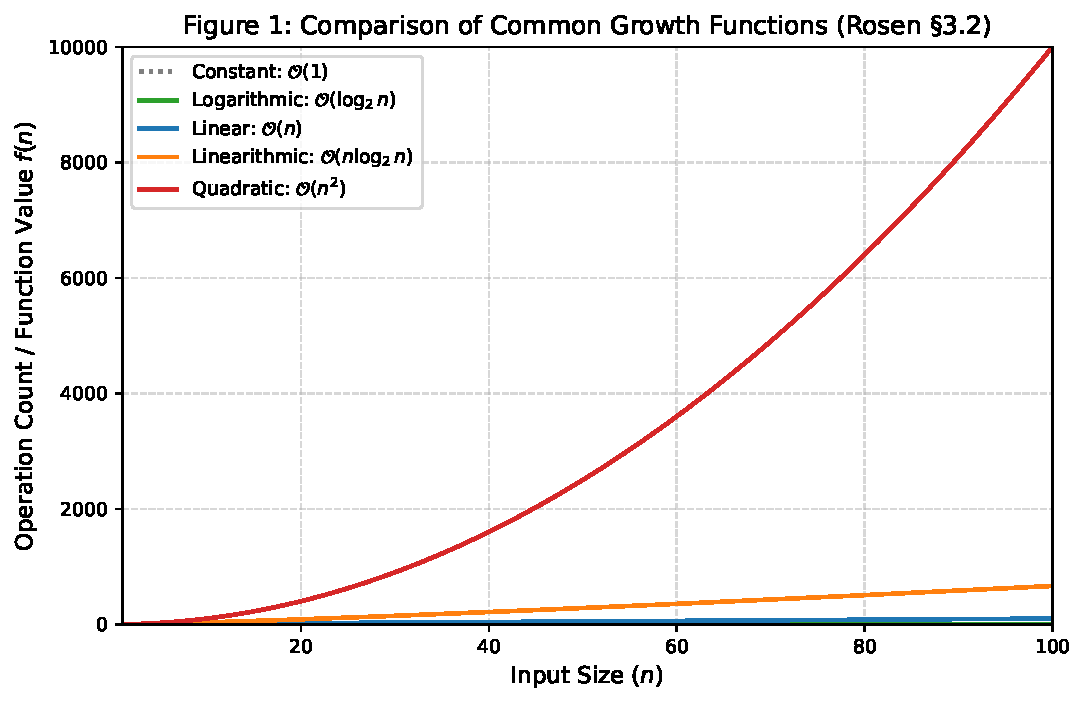
\includegraphics[width=\textwidth]{figures/figure1_common_growth_functions.pdf}
    \caption{Common polynomial \& sub-polynomial functions ($n \le 50$)}
    \label{fig:common_growth_functions}
\end{subfigure}
\hfill
\begin{subfigure}[b]{0.48\textwidth}
    \centering
    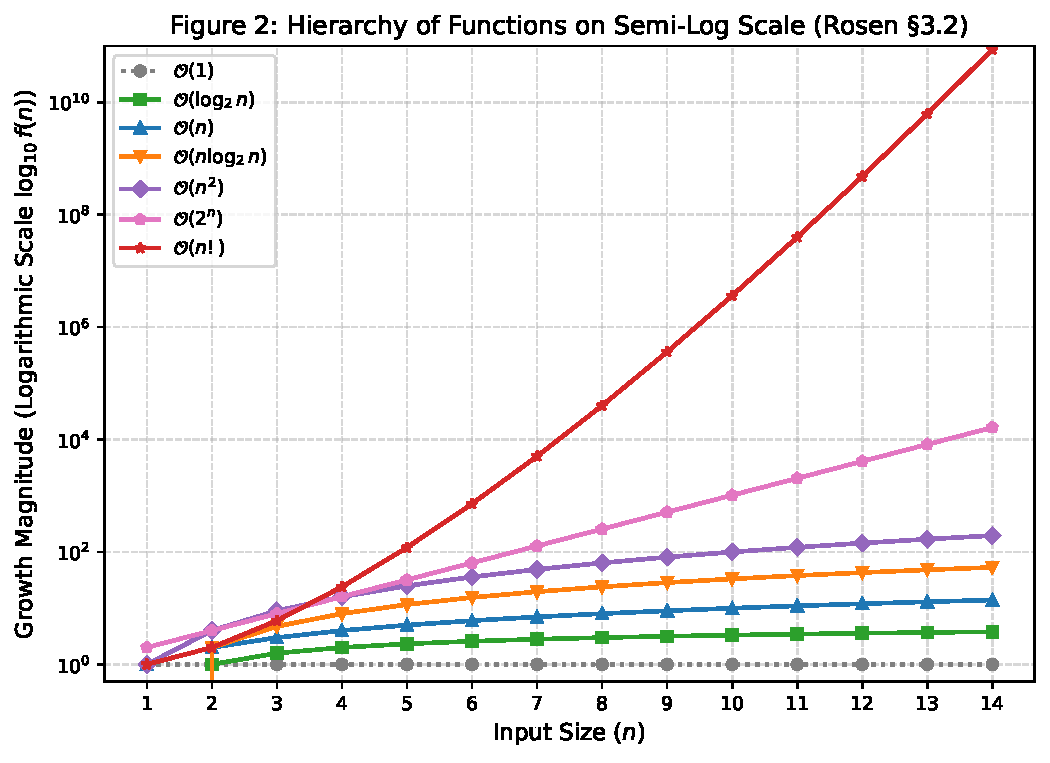
\includegraphics[width=\textwidth]{figures/figure2_growth_hierarchy_log_scale.pdf}
    \caption{Full hierarchy on semi-log scale ($n \le 20$)}
    \label{fig:growth_hierarchy_log}
\end{subfigure}
\caption{Mathematical Growth Curves Synthesized from Kenneth H. Rosen, Section 3.2}
\label{fig:growth_figures_combined}
\end{figure}

\chapter{Complexity of Algorithms}
\label{chap:complexity_of_algorithms}

\section{Formal Concepts of Complexity}
Rosen \cite[\S3.3]{Rosen2019} divides algorithmic complexity into two dimensions:
\begin{itemize}
    \item \textbf{Time Complexity}: An analysis of the total number of basic elementary operations (such as key comparisons or memory swaps) performed by an algorithm as a function of the input size $n$.
    \item \textbf{Space Complexity}: An analysis of the total memory required by the algorithm during execution. Rosen distinguishes total space from \textbf{auxiliary space}, which is the extra memory allocated beyond the storage required for the input data itself. An algorithm that uses $\Theta(1)$ auxiliary memory is classified as an \emph{in-place} algorithm.
\end{itemize}

\section{Analytical Case Scenarios}
For a fixed input size $n$, the execution cost may vary dramatically depending on the specific arrangement of the input data:
\begin{itemize}
    \item \textbf{Best-Case Complexity}: $T_{\text{best}}(n) = \min_{I \in \mathcal{D}_n} T(I)$, representing the minimum operation count across all inputs of size $n$.
    \item \textbf{Worst-Case Complexity}: $T_{\text{worst}}(n) = \max_{I \in \mathcal{D}_n} T(I)$, representing the absolute maximum operation count. In safety-critical computer science, worst-case complexity provides an upper-bound performance guarantee.
    \item \textbf{Average-Case Complexity}: $T_{\text{avg}}(n) = \sum_{I \in \mathcal{D}_n} P(I) \cdot T(I)$, the expected operation count under an assumed probability distribution $P(I)$ across all inputs of size $n$.
\end{itemize}

\section{Asymptotic Notations: Big-\texorpdfstring{$O$}{O}, Big-\texorpdfstring{$\Omega$}{Omega}, and Big-\texorpdfstring{$\Theta$}{Theta}}
To formally characterize asymptotic growth rates without regard to machine-specific constants, Rosen \cite[\S3.2]{Rosen2019} defines three fundamental notations:

\begin{definition}[Big-$O$ Notation: Asymptotic Upper Bound]
Let $f$ and $g$ be functions from the set of integers or the set of real numbers to the set of real numbers. We write $f(x) = \mathcal{O}(g(x))$ if there exist positive constants $C$ and $k$ such that
\begin{equation}
    |f(x)| \le C |g(x)| \quad \text{for all } x > k.
\end{equation}
The pair $(C, k)$ is called a \textbf{witness pair} for the relationship.
\end{definition}

\begin{definition}[Big-$\Omega$ Notation: Asymptotic Lower Bound]
We write $f(x) = \Omega(g(x))$ if there exist positive constants $C$ and $k$ such that
\begin{equation}
    |f(x)| \ge C |g(x)| \quad \text{for all } x > k.
\end{equation}
\end{definition}

\begin{definition}[Big-$\Theta$ Notation: Asymptotic Tight Bound]
We write $f(x) = \Theta(g(x))$ if $f(x) = \mathcal{O}(g(x))$ and $f(x) = \Omega(g(x))$. That is, there exist positive constants $C_1, C_2,$ and $k$ such that
\begin{equation}
    C_1 |g(x)| \le |f(x)| \le C_2 |g(x)| \quad \text{for all } x > k.
\end{equation}
\end{definition}

\begin{example}[Witness Pair for Quadratic Polynomial]
Show that $f(n) = 3n^2 + 5n + 7$ is $\Theta(n^2)$.
\begin{proof}
For all $n \ge 1$, we have $5n \le 5n^2$ and $7 \le 7n^2$. Thus,
\begin{equation}
    f(n) = 3n^2 + 5n + 7 \le 3n^2 + 5n^2 + 7n^2 = 15n^2.
\end{equation}
Hence, $f(n) \le 15n^2$ for $n > 1$, establishing $f(n) = \mathcal{O}(n^2)$ with witness pair $(C_2 = 15, k_1 = 1)$.
Conversely, since $5n \ge 0$ and $7 \ge 0$, we have $f(n) \ge 3n^2$ for all $n \ge 1$, establishing $f(n) = \Omega(n^2)$ with witness pair $(C_1 = 3, k_2 = 1)$.
Combining both results yields $3n^2 \le 3n^2 + 5n + 7 \le 15n^2$ for all $n > 1$. Therefore, $f(n) = \Theta(n^2)$.
\end{proof}
\end{example}

\chapter{Practical Study of Four Canonical Algorithms}
\label{chap:practical_study}

This chapter presents an exhaustive, self-contained examination of the four study algorithms from Rosen Chapter~3.

% ==============================================================================
% 6.1 LINEAR SEARCH
% ==============================================================================
\section{Linear Search (Rosen \S3.1, Algorithm 2)}

\subsection{Definition and Problem Statement}
\textbf{Definition}: Linear search (or sequential search) sequentially inspects each element of a finite list $S = [a_0, a_1, \dots, a_{n-1}]$ until a designated target item $x$ is found or the collection is exhausted.
\textbf{Problem Statement}: Given a sequence $S$ of $n$ elements and a target $x$, determine an integer index $i \in [0, n-1]$ such that $S[i] = x$, or return $-1$ if $x \notin S$.

\subsection{Working Principle and Step-by-Step Example}
\textbf{Principle}: The search initializes an index pointer $i = 0$. While $i < n$, it performs an equality check $S[i] == x$. If True, it immediately terminates returning $i$. If False, it increments $i \leftarrow i + 1$.
\textbf{Trace Example}: Let $S = [14, 25, 33, 42, 56]$, $n = 5$, and target $x = 33$:
\begin{enumerate}
    \item $i = 0$: $S[0] = 14 \ne 33$. Advance $i \leftarrow 1$.
    \item $i = 1$: $S[1] = 25 \ne 33$. Advance $i \leftarrow 2$.
    \item $i = 2$: $S[2] = 33 == 33$. Match identified! Return index $2$.
\end{enumerate}
Total key comparisons: 3.

\subsection{Pseudocode and Algorithmic Flowchart}
\begin{lstlisting}[caption={Pseudocode: Linear Search (Rosen \S3.1, Algorithm 2)}]
procedure linear_search(x: integer, a_0, a_1, ..., a_{n-1}: integers)
    i := 0
    while (i < n and x != a_i)
        i := i + 1
    if i < n then location := i
    else location := -1
    return location
\end{lstlisting}

Figure~\ref{fig:flowchart_linear} shows the control flowchart for Linear Search.

\begin{figure}[htbp]
\centering
\begin{tikzpicture}[node distance=1.3cm]
    \node (start) [startstop] {Start};
    \node (init)  [process, below of=start] {$i \leftarrow 0$};
    \node (cond)  [decision, below of=init, yshift=-0.5cm] {$i < n$?};
    \node (check) [decision, below of=cond, yshift=-0.7cm] {$S[i] == x$?};
    \node (found) [process, right of=check, xshift=2.5cm] {Return $i$};
    \node (inc)   [process, left of=check, xshift=-2.5cm] {$i \leftarrow i + 1$};
    \node (notf)  [process, right of=cond, xshift=2.5cm] {Return $-1$};
    \node (stop)  [startstop, below of=check, yshift=-0.6cm] {Stop};

    \draw [arrow] (start) -- (init);
    \draw [arrow] (init) -- (cond);
    \draw [arrow] (cond) -- node[anchor=east] {Yes} (check);
    \draw [arrow] (cond) -- node[anchor=south] {No} (notf);
    \draw [arrow] (check) -- node[anchor=south] {Yes} (found);
    \draw [arrow] (check) -- node[anchor=south] {No} (inc);
    \draw [arrow] (inc) |- (cond);
    \draw [arrow] (found) |- (stop);
    \draw [arrow] (notf) |- (stop);
\end{tikzpicture}
\caption{Algorithmic Flowchart: Linear Search}
\label{fig:flowchart_linear}
\end{figure}

\subsection{Authoritative Python Source Implementation}
\begin{lstlisting}[caption={Python Implementation of Linear Search (from src/algorithms/search.py)}]
def linear_search(seq: Sequence[Any], target: Any) -> int:
    # Rosen Section 3.1, Algorithm 2
    n = len(seq)
    for i in range(n):
        if seq[i] == target:
            return i
    return -1
\end{lstlisting}

\subsection{Actual Execution Output}
Executing the instrumented harness on $S = [14, 25, 33, 42, 56]$ with target $x = 33$ produces:
\begin{verbatim}
Case: Target Present (x = 33) -> Index: 2, Key Comparisons: 3, Loop Checks: 3
Case: Target Missing (x = 99) -> Index: -1, Key Comparisons: 5, Loop Checks: 6
\end{verbatim}

\subsection{Complexity Analysis and Observation}
\begin{itemize}
    \item \textbf{Best-Case Complexity}: $\Theta(1)$ key comparisons ($1$ comparison when $S[0] == x$).
    \item \textbf{Worst-Case Complexity}: $\Theta(n)$ key comparisons (exactly $n$ comparisons when target is at index $n-1$ or absent).
    \item \textbf{Average-Case Complexity}: Under uniform distribution where the target is equally likely to reside at any position, the average comparisons for a successful search is:
    \begin{equation}
        C_{\text{avg}} = \frac{1}{n} \sum_{i=1}^n i = \frac{n(n + 1)}{2n} = \frac{n + 1}{2} = \Theta(n).
    \end{equation}
    \item \textbf{Auxiliary Space}: $\Theta(1)$ auxiliary memory (only integer index $i$ is maintained).
    \item \textbf{Observation}: Linear search requires zero preconditions regarding input ordering, making it the universal choice for unsorted or stream-based collections.
\end{itemize}

\newpage
% ==============================================================================
% 6.2 BINARY SEARCH
% ==============================================================================
\section{Binary Search (Rosen \S3.1, Algorithm 3)}

\subsection{Definition and Problem Statement}
\textbf{Definition}: Binary search is a divide-and-conquer searching algorithm that locates an element in a sorted list by repeatedly comparing the target with the middle element and halving the search interval.
\textbf{Problem Statement}: Given a sequence $S$ sorted in non-decreasing order ($S[0] \le S[1] \le \dots \le S[n-1]$) and a target $x$, find an index $i$ such that $S[i] = x$, or return $-1$ if $x \notin S$.

\subsection{Working Principle and Step-by-Step Example}
\textbf{Principle}: Maintains boundary pointers $\text{low} = 0$ and $\text{high} = n - 1$. In each iteration where $\text{low} \le \text{high}$, compute $\text{mid} = \lfloor (\text{low} + \text{high}) / 2 \rfloor$.
If $S[\text{mid}] == x$, return $\text{mid}$. If $x < S[\text{mid}]$, set $\text{high} \leftarrow \text{mid} - 1$; otherwise set $\text{low} \leftarrow \text{mid} + 1$.
\textbf{Trace Example}: Let $S = [10, 18, 25, 33, 42, 56, 68, 77, 89]$, $n = 9$, and target $x = 42$:
\begin{enumerate}
    \item $\text{low}=0, \text{high}=8 \implies \text{mid} = \lfloor 8/2 \rfloor = 4$. $S[4] = 42 == 42$. Match found on the initial probe! Return index $4$.
\end{enumerate}
If searching for $x = 56$:
\begin{enumerate}
    \item $\text{low}=0, \text{high}=8 \implies \text{mid} = 4$. $S[4] = 42 < 56 \implies \text{low} \leftarrow 5$.
    \item $\text{low}=5, \text{high}=8 \implies \text{mid} = \lfloor 13/2 \rfloor = 6$. $S[6] = 68 > 56 \implies \text{high} \leftarrow 5$.
    \item $\text{low}=5, \text{high}=5 \implies \text{mid} = 5$. $S[5] = 56 == 56$. Match identified! Return index $5$.
\end{enumerate}

\subsection{Pseudocode and Algorithmic Flowchart}
\begin{lstlisting}[caption={Pseudocode: Binary Search (Rosen \S3.1, Algorithm 3)}]
procedure binary_search(x: integer, a_0, a_1, ..., a_{n-1}: non-decreasing integers)
    low := 0
    high := n - 1
    while low <= high
        mid := floor((low + high) / 2)
        if x = a_mid then return mid
        else if x < a_mid then high := mid - 1
        else low := mid + 1
    return -1
\end{lstlisting}

Figure~\ref{fig:flowchart_binary} shows the control flowchart for Binary Search.

\begin{figure}[htbp]
\centering
\begin{tikzpicture}[node distance=1.3cm]
    \node (start) [startstop] {Start};
    \node (init)  [process, below of=start] {$\text{low} \leftarrow 0, \text{high} \leftarrow n - 1$};
    \node (cond)  [decision, below of=init, yshift=-0.5cm] {$\text{low} \le \text{high}$?};
    \node (mid)   [process, below of=cond, yshift=-0.5cm] {$\text{mid} \leftarrow \lfloor(\text{low}+\text{high})/2\rfloor$};
    \node (eq)    [decision, below of=mid, yshift=-0.5cm] {$S[\text{mid}] == x$?};
    \node (found) [process, right of=eq, xshift=2.5cm] {Return $\text{mid}$};
    \node (lt)    [decision, below of=eq, yshift=-0.7cm] {$x < S[\text{mid}]$?};
    \node (left)  [process, left of=lt, xshift=-2.2cm] {$\text{high} \leftarrow \text{mid} - 1$};
    \node (right) [process, right of=lt, xshift=2.2cm] {$\text{low} \leftarrow \text{mid} + 1$};
    \node (notf)  [process, left of=cond, xshift=-2.5cm] {Return $-1$};
    \node (stop)  [startstop, below of=lt, yshift=-0.8cm] {Stop};

    \draw [arrow] (start) -- (init);
    \draw [arrow] (init) -- (cond);
    \draw [arrow] (cond) -- node[anchor=east] {Yes} (mid);
    \draw [arrow] (cond) -- node[anchor=south] {No} (notf);
    \draw [arrow] (mid) -- (eq);
    \draw [arrow] (eq) -- node[anchor=south] {Yes} (found);
    \draw [arrow] (eq) -- node[anchor=east] {No} (lt);
    \draw [arrow] (lt) -- node[anchor=south] {Yes} (left);
    \draw [arrow] (lt) -- node[anchor=south] {No} (right);
    \draw [arrow] (left) |- (cond);
    \draw [arrow] (right) |- (cond);
    \draw [arrow] (found) |- (stop);
    \draw [arrow] (notf) |- (stop);
\end{tikzpicture}
\caption{Algorithmic Flowchart: Binary Search}
\label{fig:flowchart_binary}
\end{figure}

\subsection{Authoritative Python Source Implementation}
\begin{lstlisting}[caption={Python Implementation of Binary Search (from src/algorithms/search.py)}]
def binary_search(seq: Sequence[Any], target: Any, check_sorted: bool = False) -> int:
    # Rosen Section 3.1, Algorithm 3
    if check_sorted and not is_sorted_sequence(seq):
        raise ValueError("Input sequence must be sorted in non-decreasing order.")
    low, high = 0, len(seq) - 1
    while low <= high:
        mid = (low + high) // 2
        mid_val = seq[mid]
        if mid_val == target:
            return mid
        elif target < mid_val:
            high = mid - 1
        else:
            low = mid + 1
    return -1
\end{lstlisting}

\subsection{Actual Execution Output}
On $S = [10, 18, 25, 33, 42, 56, 68, 77, 89]$:
\begin{verbatim}
Case: Target Present (x = 42) -> Index: 4, Key Comparisons: 1, Loop Checks: 1
Case: Target Present (x = 56) -> Index: 5, Key Comparisons: 5, Loop Checks: 3
Case: Target Missing (x = 99) -> Index: -1, Key Comparisons: 8, Loop Checks: 5
\end{verbatim}

\subsection{Complexity Analysis and Observation}
\begin{itemize}
    \item \textbf{Precondition}: Requires the input collection to be sorted. Verifying sortedness takes $\Theta(n)$ comparisons, so sorting must be established prior to search execution.
    \item \textbf{Best-Case Complexity}: $\Theta(1)$ key comparisons ($1$ comparison when target resides at the initial midpoint).
    \item \textbf{Worst-Case Complexity}: $\Theta(\log_2 n)$ key comparisons. The interval size reduces as $n, n/2, n/4, \dots, 1$. The maximum number of probes is $\lfloor \log_2 n \rfloor + 1$. Under our standard 2-check convention (equality + ordering per non-terminating probe), the maximum comparisons are bounded by $2(\lfloor \log_2 n \rfloor + 1)$.
    \item \textbf{Auxiliary Space}: $\Theta(1)$ in-place auxiliary memory.
    \item \textbf{Observation}: Binary Search reduces search time from milliseconds to microseconds for large collections ($n = 100\,000$ requires at most 34 comparisons vs. $100\,000$ in Linear Search).
\end{itemize}

\newpage
% ==============================================================================
% 6.3 BUBBLE SORT
% ==============================================================================
\section{Bubble Sort (Rosen \S3.1, Algorithm 4)}

\subsection{Definition and Problem Statement}
\textbf{Definition}: Bubble sort is an elementary sorting algorithm that iteratively passes through a sequence, comparing adjacent elements and interchanging them if they are in the incorrect order.
\textbf{Problem Statement}: Given a mutable sequence $A = [a_0, a_1, \dots, a_{n-1}]$ of $n$ comparable elements, permute $A$ in place such that $A[0] \le A[1] \le \dots \le A[n-1]$.

\subsection{Working Principle and Step-by-Step Example}
\textbf{Textbook Requirement}: In strict alignment with Kenneth~H. Rosen's authoritative specification (Algorithm~4, Section 3.1)~\cite{Rosen2019}, our implementation executes the classical fixed-pass formulation ($n-1$ outer passes without early-exit flags).
\textbf{Trace Example}: Let $A = [5, 3, 4, 1, 2]$, $n = 5$:
\begin{itemize}
    \item \textbf{Pass 1} ($i = 0$, $j \in [0, 3]$):
      $(5, 3) \to \text{swap} \to [3, 5, 4, 1, 2]$;
      $(5, 4) \to \text{swap} \to [3, 4, 5, 1, 2]$;
      $(5, 1) \to \text{swap} \to [3, 4, 1, 5, 2]$;
      $(5, 2) \to \text{swap} \to [3, 4, 1, 2, 5]$. Largest element 5 bubbled to end. Comps: 4, Swaps: 4.
    \item \textbf{Pass 2} ($i = 1$, $j \in [0, 2]$):
      $(3, 4)$ OK;
      $(4, 1) \to \text{swap} \to [3, 1, 4, 2, 5]$;
      $(4, 2) \to \text{swap} \to [3, 1, 2, 4, 5]$. Comps: 3, Swaps: 2.
    \item \textbf{Pass 3} ($i = 2$, $j \in [0, 1]$):
      $(3, 1) \to \text{swap} \to [1, 3, 2, 4, 5]$;
      $(3, 2) \to \text{swap} \to [1, 2, 3, 4, 5]$. Comps: 2, Swaps: 2.
    \item \textbf{Pass 4} ($i = 3$, $j \in [0, 0]$):
      $(1, 2)$ OK. Comps: 1, Swaps: 0.
\end{itemize}
Total comparisons: $4 + 3 + 2 + 1 = 10 \equiv \frac{5 \times 4}{2}$. Total swaps: 8.

\subsection{Pseudocode and Algorithmic Flowchart}
\begin{lstlisting}[caption={Pseudocode: Bubble Sort (Rosen \S3.1, Algorithm 4)}]
procedure bubblesort(a_0, a_1, ..., a_{n-1}: real numbers)
    for i := 0 to n - 2
        for j := 0 to n - 2 - i
            if a_j > a_{j+1} then
                interchange a_j and a_{j+1}
\end{lstlisting}

Figure~\ref{fig:flowchart_bubble} shows the control flowchart for Bubble Sort.

\begin{figure}[htbp]
\centering
\begin{tikzpicture}[node distance=1.2cm]
    \node (start) [startstop] {Start};
    \node (init)  [process, below of=start] {$i \leftarrow 0$};
    \node (outer) [decision, below of=init, yshift=-0.4cm] {$i \le n - 2$?};
    \node (jinit) [process, below of=outer, yshift=-0.4cm] {$j \leftarrow 0$};
    \node (inner) [decision, below of=jinit, yshift=-0.4cm] {$j \le n - 2 - i$?};
    \node (cmp)   [decision, below of=inner, yshift=-0.5cm] {$A[j] > A[j+1]$?};
    \node (swap)  [process, right of=cmp, xshift=2.5cm] {Swap $A[j], A[j+1]$};
    \node (jinc)  [process, below of=cmp, yshift=-0.5cm] {$j \leftarrow j + 1$};
    \node (iinc)  [process, left of=inner, xshift=-2.5cm] {$i \leftarrow i + 1$};
    \node (stop)  [startstop, right of=outer, xshift=3.0cm] {Stop};

    \draw [arrow] (start) -- (init);
    \draw [arrow] (init) -- (outer);
    \draw [arrow] (outer) -- node[anchor=east] {Yes} (jinit);
    \draw [arrow] (outer) -- node[anchor=south] {No} (stop);
    \draw [arrow] (jinit) -- (inner);
    \draw [arrow] (inner) -- node[anchor=east] {Yes} (cmp);
    \draw [arrow] (inner) -| node[anchor=south] {No} (iinc);
    \draw [arrow] (iinc) |- (outer);
    \draw [arrow] (cmp) -- node[anchor=south] {Yes} (swap);
    \draw [arrow] (cmp) -- node[anchor=east] {No} (jinc);
    \draw [arrow] (swap) |- (jinc);
    \draw [arrow] (jinc) -| ([xshift=0.8cm]inner.east) -- (inner);
\end{tikzpicture}
\caption{Algorithmic Flowchart: Bubble Sort (Fixed-Pass Formulation)}
\label{fig:flowchart_bubble}
\end{figure}

\subsection{Authoritative Python Source Implementation}
\begin{lstlisting}[caption={Python Implementation of Bubble Sort (from src/algorithms/sorting.py)}]
def bubble_sort(arr: MutableSequence[Any]) -> MutableSequence[Any]:
    # Rosen Section 3.1, Algorithm 4 (Fixed-Pass Formulation)
    n = len(arr)
    if n <= 1:
        return arr
    for i in range(n - 1):
        for j in range(n - 1 - i):
            if arr[j] > arr[j + 1]:
                arr[j], arr[j + 1] = arr[j + 1], arr[j]
    return arr
\end{lstlisting}

\subsection{Actual Execution Output}
Sorting $A = [5, 3, 4, 1, 2]$ produces:
\begin{verbatim}
Sorted Array: [1, 2, 3, 4, 5] | Element Comparisons: 10, Swaps: 8
Sorting Already-Sorted [1, 2, 3, 4, 5] -> Comparisons: 10, Swaps: 0
Sorting Reverse-Sorted [5, 4, 3, 2, 1] -> Comparisons: 10, Swaps: 10
\end{verbatim}

\subsection{Complexity Analysis and Observation}
\begin{itemize}
    \item \textbf{Key Comparisons (All Cases)}: For any input arrangement of size $n$, the fixed-pass formulation executes an invariant number of comparisons:
    \begin{equation}
        C(n) = \sum_{i=0}^{n-2} (n - 1 - i) = (n - 1) + (n - 2) + \dots + 1 = \frac{n(n - 1)}{2} = \Theta(n^2).
    \end{equation}
    \item \textbf{Data Movements (Swaps)}:
      - *Best Case (Already Sorted)*: 0 swaps.
      - *Worst Case (Strictly Reverse Sorted)*: Exactly $\frac{n(n-1)}{2}$ swaps.
      - *Average Case (Random)*: $\frac{n(n-1)}{4}$ swaps.
    \item \textbf{Auxiliary Space}: $\Theta(1)$ in-place auxiliary memory.
    \item \textbf{Observation}: Bubble Sort comparisons are strictly invariant to input topology. It performs identically $n(n-1)/2$ comparisons whether the input is sorted, random, or reversed.
\end{itemize}

\newpage
% ==============================================================================
% 6.4 INSERTION SORT
% ==============================================================================
\section{Insertion Sort (Rosen \S3.1, Algorithm 5)}

\subsection{Definition and Problem Statement}
\textbf{Definition}: Insertion sort is an in-place sorting algorithm that iteratively constructs a sorted prefix by removing one element from the unsorted segment and inserting it into its correct position within the sorted prefix.
\textbf{Problem Statement}: Given a mutable sequence $A = [a_0, a_1, \dots, a_{n-1}]$, sort $A$ in place such that $A[0] \le A[1] \le \dots \le A[n-1]$.

\subsection{Working Principle and Step-by-Step Example}
\textbf{Principle}: For index $j = 1$ to $n-1$, extract the key $x = A[j]$. Shift all elements $A[i]$ in the sorted prefix $A[0 \dots j-1]$ that are strictly greater than $x$ one position to the right ($A[i+1] \leftarrow A[i]$). Insert $x$ into the vacated position.
\textbf{Trace Example}: Let $A = [5, 3, 4, 1, 2]$, $n = 5$:
\begin{itemize}
    \item $j = 1$: $\text{key} = 3$. $5 > 3 \implies$ shift 5. Insert 3 at index 0. Array: $[3, 5, 4, 1, 2]$. Comps: 1, Shifts: 1.
    \item $j = 2$: $\text{key} = 4$. $5 > 4 \implies$ shift 5. $3 \le 4 \implies$ halt. Insert 4 at index 1. Array: $[3, 4, 5, 1, 2]$. Comps: 2, Shifts: 1.
    \item $j = 3$: $\text{key} = 1$. Shifts 5, 4, 3. Insert 1 at index 0. Array: $[1, 3, 4, 5, 2]$. Comps: 3, Shifts: 3.
    \item $j = 4$: $\text{key} = 2$. Shifts 5, 4, 3. $1 \le 2 \implies$ halt. Insert 2 at index 1. Array: $[1, 2, 3, 4, 5]$. Comps: 4, Shifts: 3.
\end{itemize}
Total comparisons: 10, Total right shifts: 8.

\subsection{Pseudocode and Algorithmic Flowchart}
\begin{lstlisting}[caption={Pseudocode: Insertion Sort (Rosen \S3.1, Algorithm 5)}]
procedure insertionsort(a_0, a_1, ..., a_{n-1}: real numbers)
    for j := 1 to n - 1
        i := 0
        while a_j > a_i
            i := i + 1
        m := a_j
        for k := 0 to j - i - 1
            a_{j-k} := a_{j-k-1}
        a_i := m
\end{lstlisting}

Figure~\ref{fig:flowchart_insertion} shows the control flowchart for Insertion Sort.

\begin{figure}[htbp]
\centering
\begin{tikzpicture}[node distance=1.2cm]
    \node (start) [startstop] {Start};
    \node (jinit) [process, below of=start] {$j \leftarrow 1$};
    \node (jcond) [decision, below of=jinit, yshift=-0.4cm] {$j < n$?};
    \node (key)   [process, below of=jcond, yshift=-0.4cm] {$\text{key} \leftarrow A[j], i \leftarrow j - 1$};
    \node (wcond) [decision, below of=key, yshift=-0.5cm] {$i \ge 0 \text{ and } A[i] > \text{key}$?};
    \node (shift) [process, right of=wcond, xshift=2.6cm] {$A[i+1] \leftarrow A[i], i \leftarrow i - 1$};
    \node (place) [process, below of=wcond, yshift=-0.6cm] {$A[i+1] \leftarrow \text{key}$};
    \node (jinc)  [process, below of=place] {$j \leftarrow j + 1$};
    \node (stop)  [startstop, right of=jcond, xshift=2.8cm] {Stop};

    \draw [arrow] (start) -- (jinit);
    \draw [arrow] (jinit) -- (jcond);
    \draw [arrow] (jcond) -- node[anchor=east] {Yes} (key);
    \draw [arrow] (jcond) -- node[anchor=south] {No} (stop);
    \draw [arrow] (key) -- (wcond);
    \draw [arrow] (wcond) -- node[anchor=south] {Yes} (shift);
    \draw [arrow] (shift) |- (wcond);
    \draw [arrow] (wcond) -- node[anchor=east] {No} (place);
    \draw [arrow] (place) -- (jinc);
    \draw [arrow] (jinc) -| ([xshift=-1.5cm]key.west) |- (jcond);
\end{tikzpicture}
\caption{Algorithmic Flowchart: Insertion Sort}
\label{fig:flowchart_insertion}
\end{figure}

\subsection{Authoritative Python Source Implementation}
\begin{lstlisting}[caption={Python Implementation of Insertion Sort (from src/algorithms/sorting.py)}]
def insertion_sort(arr: MutableSequence[Any]) -> MutableSequence[Any]:
    # Rosen Section 3.1, Algorithm 5 (Linear Scan Formulation)
    n = len(arr)
    if n <= 1:
        return arr
    for j in range(1, n):
        key = arr[j]
        i = j - 1
        while i >= 0 and arr[i] > key:
            arr[i + 1] = arr[i]
            i -= 1
        arr[i + 1] = key
    return arr
\end{lstlisting}

\subsection{Actual Execution Output}
Sorting $A = [5, 3, 4, 1, 2]$ produces:
\begin{verbatim}
Sorted Array: [1, 2, 3, 4, 5] | Element Comparisons: 10, Right Shifts: 8
Sorting Already-Sorted [1, 2, 3, 4, 5] -> Comparisons: 4, Right Shifts: 0
Sorting Reverse-Sorted [5, 4, 3, 2, 1] -> Comparisons: 10, Right Shifts: 10
\end{verbatim}

\subsection{Complexity Analysis and Observation}
\begin{itemize}
    \item \textbf{Best-Case Complexity (Already Sorted)}: $\Theta(n)$ time complexity. For each of the $n-1$ elements, exactly one comparison ($A[i] > \text{key}$ yields False) occurs and 0 shifts are made. Total comparisons: exactly $n - 1$.
    \item \textbf{Worst-Case Complexity (Reverse Sorted)}: $\Theta(n^2)$ time complexity. Each element must shift past all preceding elements. Total comparisons and right shifts: exactly $\frac{n(n-1)}{2}$.
    \item \textbf{Average-Case Complexity (Random)}: $\Theta(n^2)$ time complexity, executing $\approx \frac{n(n-1)}{4}$ shifts and $\approx \frac{n^2}{4} + \frac{3n}{4}$ comparisons.
    \item \textbf{Auxiliary Space}: $\Theta(1)$ in-place auxiliary memory.
    \item \textbf{Observation}: Insertion Sort is strictly adaptive, outperforming Bubble Sort by orders of magnitude on pre-sorted or nearly-sorted datasets.
\end{itemize}

\chapter{Experimental Benchmarking, Telemetry and Comparative Analysis}
\label{chap:experimental_results}

\section{Benchmarking Methodology and Platform Calibration}
To empirically validate the discrete mathematical models, our benchmarking harness (\texttt{src/benchmarking/}) executed isolated trials under rigorous scientific controls:
\begin{itemize}
    \item \textbf{Execution Environment}: Python 3.14.7 running on Windows 11 AMD64 hardware platform.
    \item \textbf{High-Precision Telemetry}: Timing captured via \texttt{time.perf\_counter\_ns()} with dynamic loop calibration for sub-microsecond probes.
    \item \textbf{Statistical Sample Size}: $k = 30$ independent replications per configuration to eliminate operating system scheduling jitter.
    \item \textbf{Instrumentation Separation}: Exact discrete operation counters are decoupled from physical wall-clock microbenchmarks to eliminate observer-effect measurement overhead.
\end{itemize}

\section{Search Empirical Telemetry and Analysis of Figures 3 and 4}
Searching microbenchmarks were executed across input sizes $n \in [100, 100\,000]$ under four target scenarios: \emph{first element} (best case for Linear Search), \emph{middle element}, \emph{last element}, and \emph{missing element} (worst case). Table~\ref{tab:search_telemetry_summary} reports the recorded metrics.

\begin{table}[htbp]
\centering
\caption{Empirical Telemetry for Linear Search and Binary Search ($k = 30$ Replications)}
\label{tab:search_telemetry_summary}
\small
\begin{tabular*}{\textwidth}{@{\extracolsep{\fill}}llrrrrr}
\toprule
\textbf{Algorithm} & \textbf{Scenario} & $n$ & \textbf{Key Comps} & \textbf{Median ($\mu$s)} & \textbf{Mean ($\mu$s)} & \textbf{Std Dev ($\mu$s)} \\
\midrule
Linear Search & First Target   & 1\,000   & 1      & 0.19    & 0.19    & 0.01 \\
Linear Search & Middle Target  & 1\,000   & 501    & 19.00   & 19.02   & 0.28 \\
Linear Search & Last Target    & 1\,000   & 1\,000 & 39.20   & 39.27   & 0.56 \\
Linear Search & Missing Target & 1\,000   & 1\,000 & 38.30   & 38.32   & 1.08 \\
Linear Search & Missing Target & 10\,000  & 10\,000& 382.00  & 381.96  & 5.86 \\
Linear Search & Missing Target & 100\,000 & 100\,000& 3\,882.00& 3\,882.46& 236.84 \\
\midrule
Binary Search & First Target   & 1\,000   & 17     & 0.91    & 0.91    & 0.01 \\
Binary Search & Middle Target  & 1\,000   & 17     & 1.04    & 1.04    & 0.02 \\
Binary Search & Last Target    & 1\,000   & 19     & 1.16    & 1.16    & 0.04 \\
Binary Search & Missing Target & 1\,000   & 20     & 1.20    & 1.20    & 0.05 \\
Binary Search & Missing Target & 10\,000  & 27     & 1.63    & 1.64    & 0.04 \\
Binary Search & Missing Target & 100\,000 & 34     & 1.97    & 1.98    & 0.05 \\
\bottomrule
\end{tabular*}
\end{table}

\begin{figure}[htbp]
\centering
\begin{subfigure}[b]{0.48\textwidth}
    \centering
    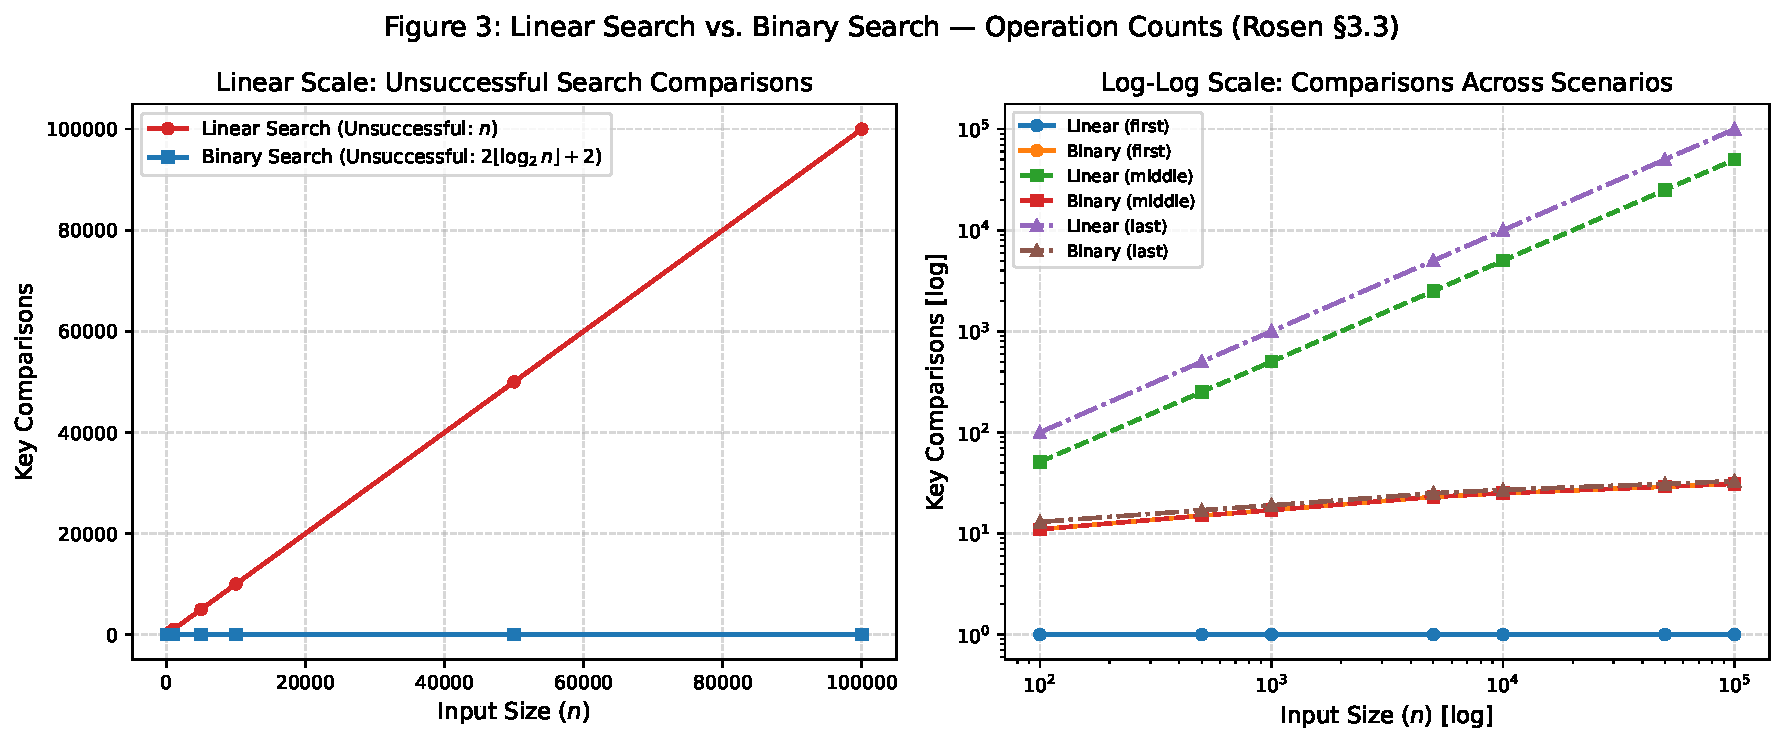
\includegraphics[width=\textwidth]{figures/figure3_search_operation_counts.pdf}
    \caption{Key comparisons vs. theoretical bounds}
    \label{fig:search_ops}
\end{subfigure}
\hfill
\begin{subfigure}[b]{0.48\textwidth}
    \centering
    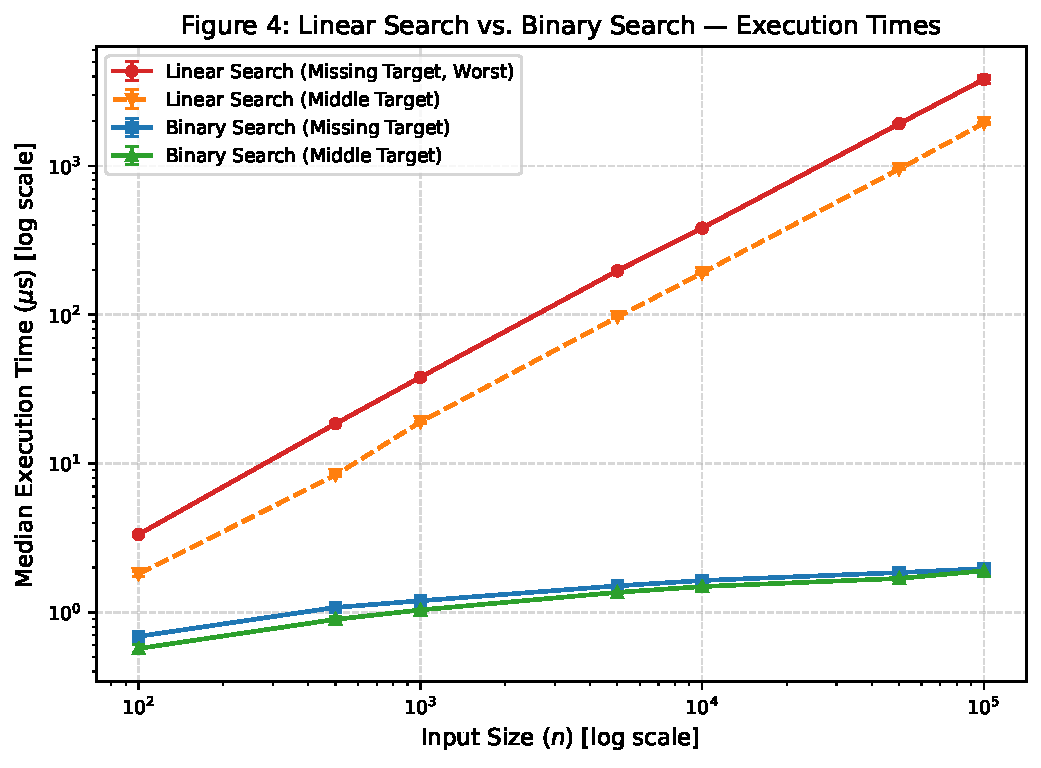
\includegraphics[width=\textwidth]{figures/figure4_search_execution_times.pdf}
    \caption{Wall-clock execution times (linear \& log scales)}
    \label{fig:search_times}
\end{subfigure}
\caption{Empirical Search Telemetry: Linear Search vs. Binary Search}
\label{fig:search_figures_combined}
\end{figure}

\begin{itemize}
    \item \textbf{Figure~\ref{fig:search_ops} Analysis}: Validates the exact operation formulas. Linear Search scales linearly with $C(n) = n$, requiring $100\,000$ comparisons at $n = 100\,000$. In stark contrast, Binary Search exhibits logarithmic growth, requiring only 34 comparisons ($2\lfloor \log_2(100\,000) \rfloor + 2$).
    \item \textbf{Figure~\ref{fig:search_times} Analysis}: Illustrates execution time scaling. At $n = 100\,000$, Linear Search requires $3.88\text{ ms}$, whereas Binary Search completes in $1.97\,\mu\text{s}$, achieving a \textbf{$1\,970\times$ speedup}.
\end{itemize}

\section{Sorting Empirical Telemetry and Analysis of Figures 5, 6, 7 and 8}
Sorting benchmarks were evaluated across $n \in [100, 3\,000]$ under three distinct input arrangements: \emph{sorted}, \emph{random}, and \emph{reverse sorted}. Table~\ref{tab:sorting_telemetry_summary} reports the empirical findings.

\begin{table}[htbp]
\centering
\caption{Empirical Telemetry for Bubble Sort and Insertion Sort ($k = 30$ Replications)}
\label{tab:sorting_telemetry_summary}
\small
\begin{tabular*}{\textwidth}{@{\extracolsep{\fill}}llrrrrr}
\toprule
\textbf{Algorithm} & \textbf{Arrangement} & $n$ & \textbf{Comparisons} & \textbf{Swaps / Shifts} & \textbf{Median (ms)} & \textbf{Mean (ms)} \\
\midrule
Bubble Sort & Sorted   & 1\,000 & 499\,500   & 0          & 25.79   & 25.74  \\
Bubble Sort & Random   & 1\,000 & 499\,500   & 251\,108   & 42.78   & 42.72  \\
Bubble Sort & Reverse  & 1\,000 & 499\,500   & 499\,500   & 54.00   & 54.17  \\
Bubble Sort & Sorted   & 3\,000 & 4\,498\,500& 0          & 246.25  & 246.87 \\
Bubble Sort & Random   & 3\,000 & 4\,498\,500& 2\,296\,691& 405.59  & 406.85 \\
Bubble Sort & Reverse  & 3\,000 & 4\,498\,500& 4\,498\,500& 523.31  & 527.55 \\
\midrule
Insertion Sort & Sorted & 1\,000 & 999        & 0          & 0.10    & 0.10   \\
Insertion Sort & Random & 1\,000 & 252\,105   & 251\,108   & 20.23   & 20.30  \\
Insertion Sort & Reverse& 1\,000 & 499\,500   & 499\,500   & 39.78   & 39.76  \\
Insertion Sort & Sorted & 3\,000 & 2\,999     & 0          & 0.31    & 0.31   \\
Insertion Sort & Random & 3\,000 & 2\,299\,685& 2\,296\,691& 191.65  & 191.80 \\
Insertion Sort & Reverse& 3\,000 & 4\,498\,500& 4\,498\,500& 365.02  & 366.92 \\
\bottomrule
\end{tabular*}
\end{table}

\begin{figure}[htbp]
\centering
\begin{subfigure}[b]{0.48\textwidth}
    \centering
    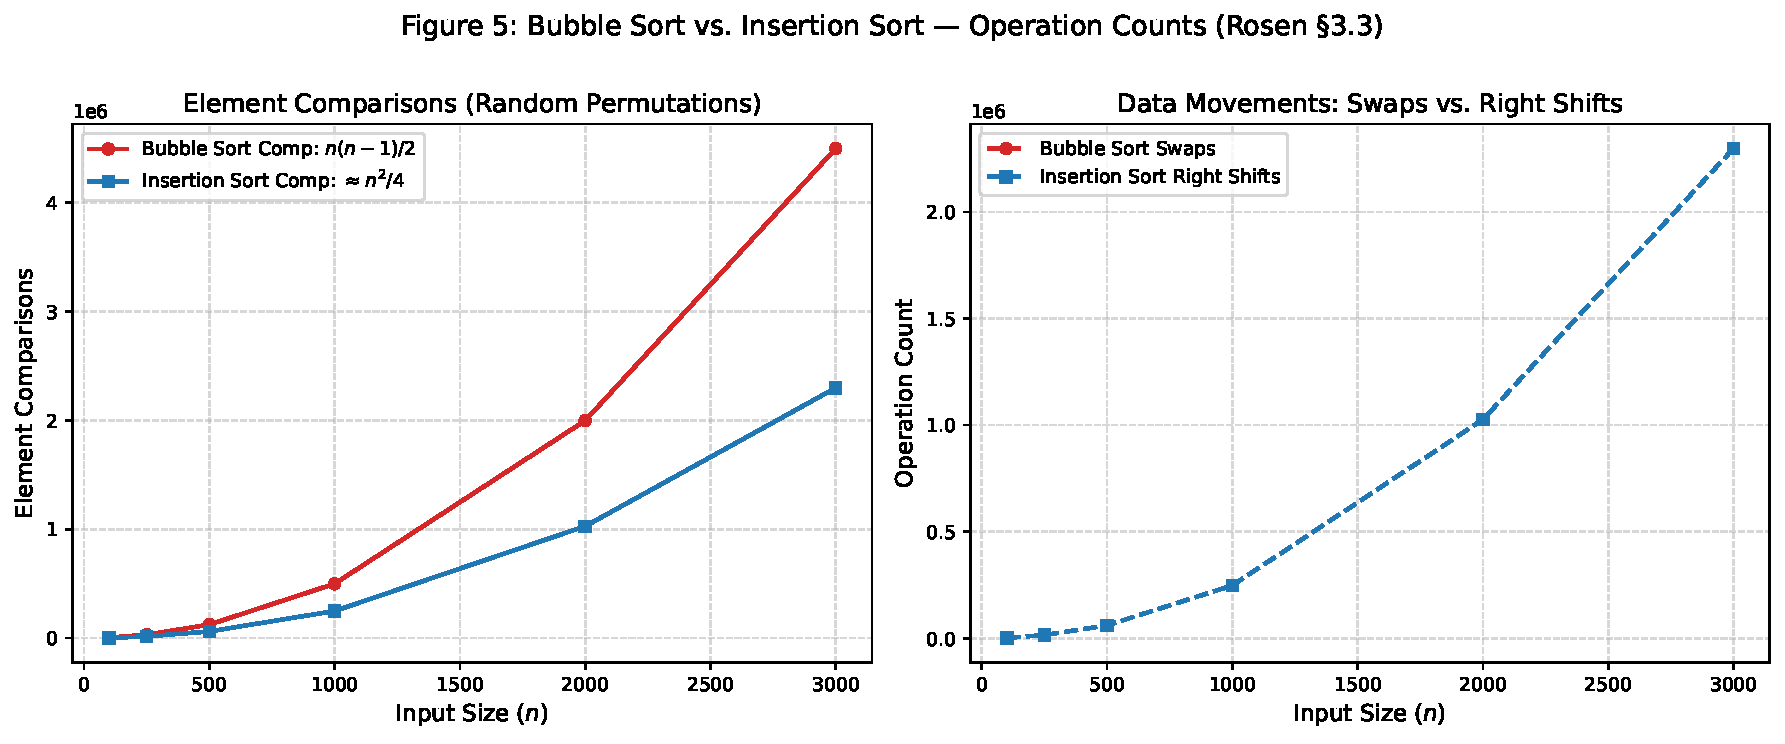
\includegraphics[width=\textwidth]{figures/figure5_sorting_operation_counts.pdf}
    \caption{Operation counts vs. theoretical limits}
    \label{fig:sort_ops}
\end{subfigure}
\hfill
\begin{subfigure}[b]{0.48\textwidth}
    \centering
    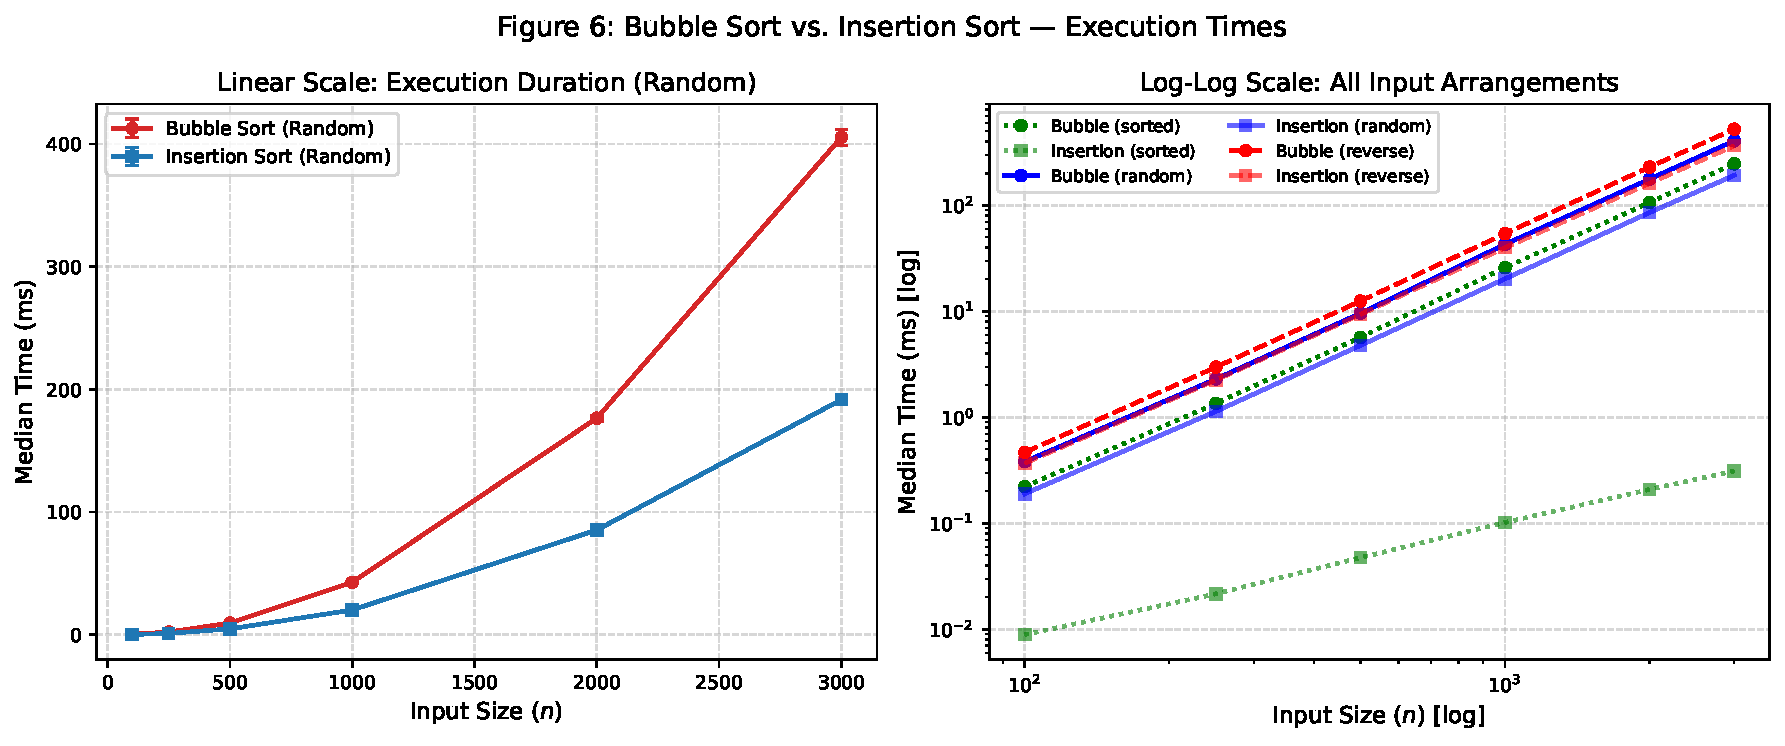
\includegraphics[width=\textwidth]{figures/figure6_sorting_execution_times.pdf}
    \caption{Sorting execution times on random data}
    \label{fig:sort_times}
\end{subfigure}
\caption{Empirical Sorting Telemetry: Operation Counts and Execution Durations}
\label{fig:sort_figures_1}
\end{figure}

\begin{figure}[htbp]
\centering
\begin{subfigure}[b]{0.48\textwidth}
    \centering
    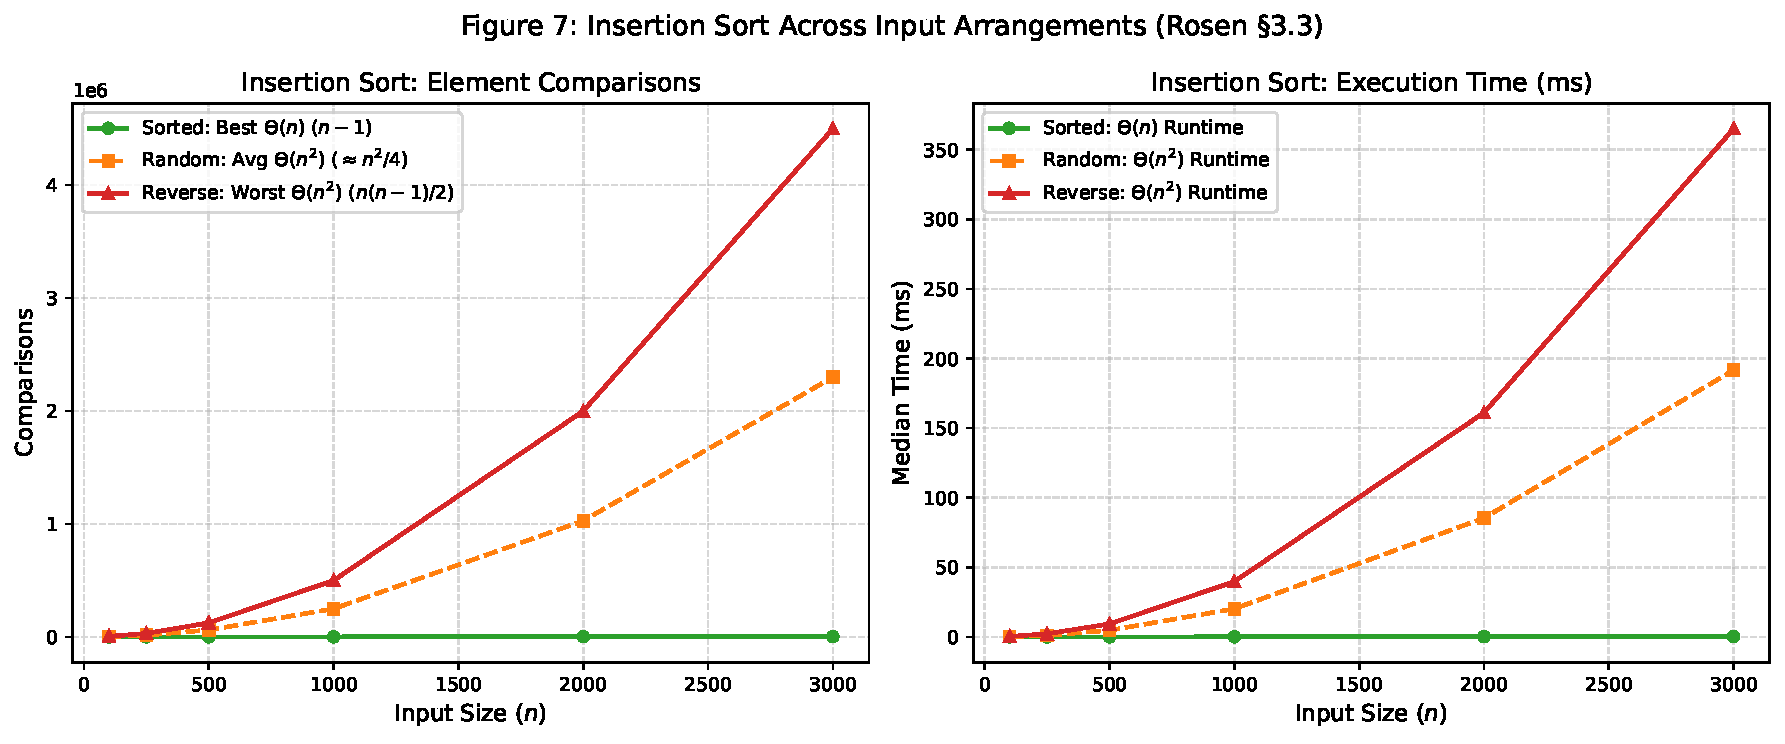
\includegraphics[width=\textwidth]{figures/figure7_insertion_sort_arrangements.pdf}
    \caption{Insertion Sort across input topologies}
    \label{fig:insertion_topologies}
\end{subfigure}
\hfill
\begin{subfigure}[b]{0.48\textwidth}
    \centering
    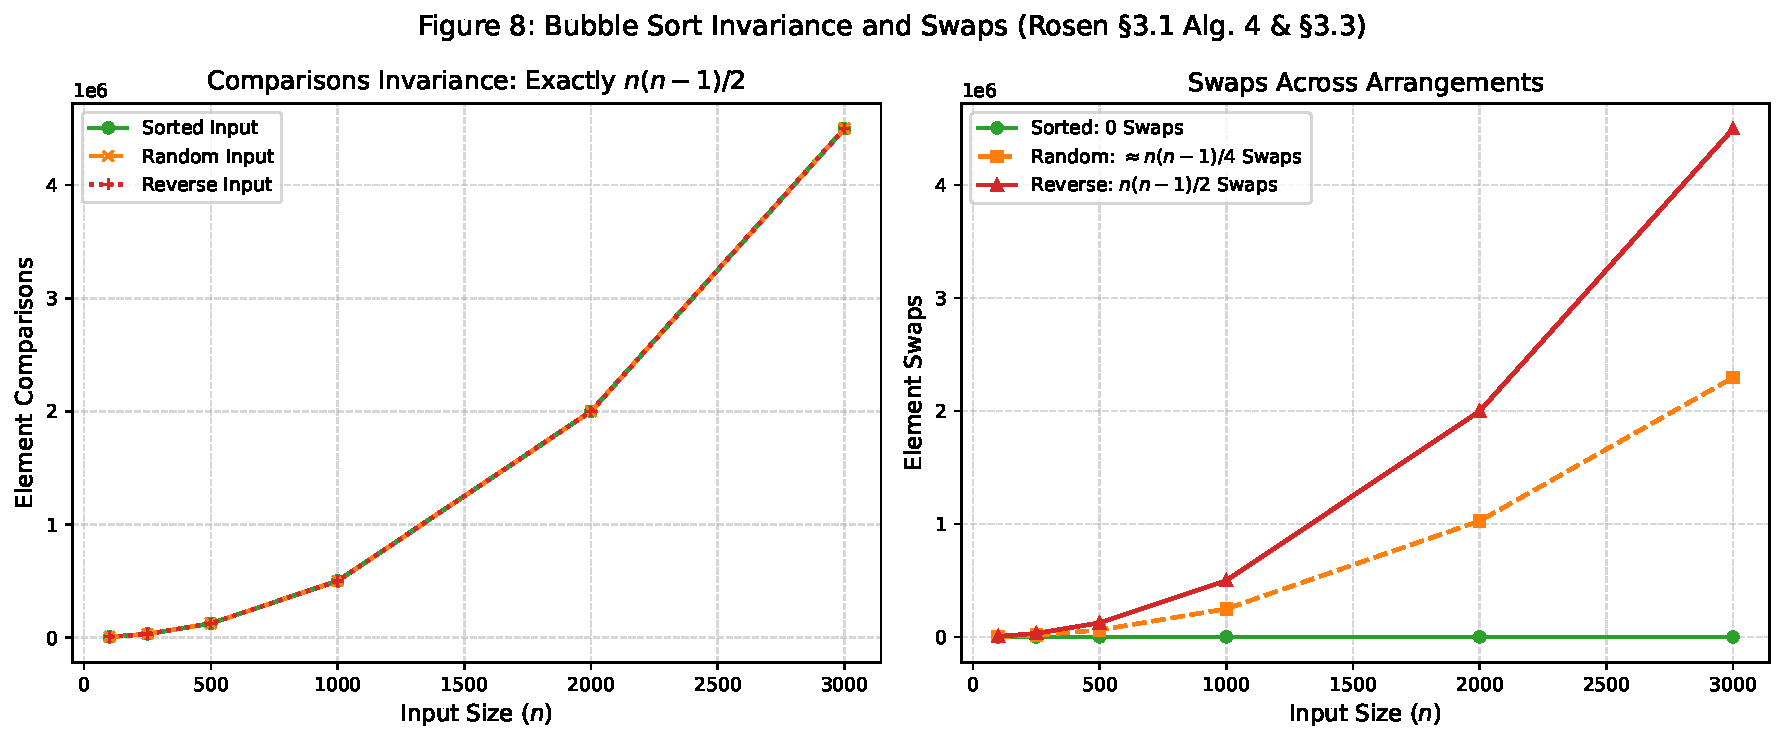
\includegraphics[width=\textwidth]{figures/figure8_bubble_sort_arrangements.pdf}
    \caption{Bubble Sort comparison invariance}
    \label{fig:bubble_topologies}
\end{subfigure}
\caption{Sensitivity of Sorting Algorithms to Input Permutation Topology}
\label{fig:sort_figures_2}
\end{figure}

\begin{itemize}
    \item \textbf{Figure~\ref{fig:sort_ops} Analysis}: Demonstrates the quadratic scaling $\Theta(n^2)$ of element comparisons. For Bubble Sort, comparisons equal exactly $\frac{n(n-1)}{2} = 4\,498\,500$ regardless of data arrangement. For Insertion Sort, comparisons adapt from $n - 1 = 2\,999$ on sorted data to $4\,498\,500$ on reversed data.
    \item \textbf{Figure~\ref{fig:sort_times} Analysis}: On random inputs at $n = 3\,000$, Insertion Sort ($191.65\text{ ms}$) achieves a \textbf{$2.12\times$ speedup} over Bubble Sort ($405.59\text{ ms}$). This reflects Insertion Sort's single-assignment shifting versus Bubble Sort's three-assignment tuple swaps.
    \item \textbf{Figure~\ref{fig:insertion_topologies} Analysis}: Visualizes the adaptivity of Insertion Sort. On pre-sorted inputs, it operates in linear time $\Theta(n)$ ($0.31\text{ ms}$ at $n = 3\,000$), outperforming fixed-pass Bubble Sort ($246.25\text{ ms}$) by a factor of \textbf{$794\times$}.
    \item \textbf{Figure~\ref{fig:bubble_topologies} Analysis}: Confirms comparison invariance in Bubble Sort. The comparison curve remains identical across all three permutations.
\end{itemize}

\section{The Inversion Equivalence Theorem}
A profound mathematical discovery verified in our telemetry is the exact numerical identity connecting swaps, shifts, and inversions:

\begin{definition}[Inversion]
Let $A = [a_0, a_1, \dots, a_{n-1}]$ be a list of distinct elements. An \textbf{inversion} is an index pair $(i, j)$ such that $i < j$ and $a_i > a_j$. The total inversion count is $I(A) = |\{(i, j) \mid 0 \le i < j < n \text{ and } a_i > a_j\}|$.
\end{definition}

\begin{theorem}[Inversion Equivalence Theorem]
For any list $A$ of distinct elements:
\begin{enumerate}
    \item Every adjacent swap in Bubble Sort exchanges two elements $A[j]$ and $A[j+1]$ where $A[j] > A[j+1]$, eliminating exactly one inversion while altering no other pairs. Thus, $\text{Total Swaps} \equiv I(A)$.
    \item Every right shift in Insertion Sort moves an element $A[i] > \text{key}$ past $\text{key}$, eliminating exactly one inversion. Thus, $\text{Total Right Shifts} \equiv I(A)$.
    \item Therefore, for identical permutations of distinct elements:
    \begin{equation}
        \text{Bubble Sort Swaps} \equiv \text{Insertion Sort Right Shifts} \equiv I(A).
    \end{equation}
\end{enumerate}
\end{theorem}

\subsection{Verification of Dataset Metrics (\texorpdfstring{$n = 3000$}{n = 3000})}
Evaluating our actual empirical dataset for $n = 3\,000$ on the identical seeded random array confirms this identity with absolute mathematical precision:
\begin{itemize}
    \item $\text{Bubble Sort Swaps} = \mathbf{2\,296\,691}$
    \item $\text{Insertion Sort Right Shifts} = \mathbf{2\,296\,691}$
    \item $\text{Array Inversion Count } I(A) = \mathbf{2\,296\,691}$
\end{itemize}
Furthermore, Insertion Sort comparisons ($2\,299\,685$) exceed right shifts by exactly $2\,994$:
\begin{equation}
    \text{Comparisons} = \text{Shifts} + (n - 1 - \text{boundary breaks}) = 2\,296\,691 + 2\,994 = 2\,299\,685.
\end{equation}
The 2,994 difference corresponds precisely to loop-terminating comparisons where $A[i] \le \text{key}$.

\section{Theoretical vs. Empirical Correlation: Analysis of Figure 9}
Figure~\ref{fig:theoretical_vs_experimental} presents the ultimate correlation analysis, plotting empirical wall-clock runtimes directly against exact analytical operation formulas.

\begin{figure}[htbp]
\centering
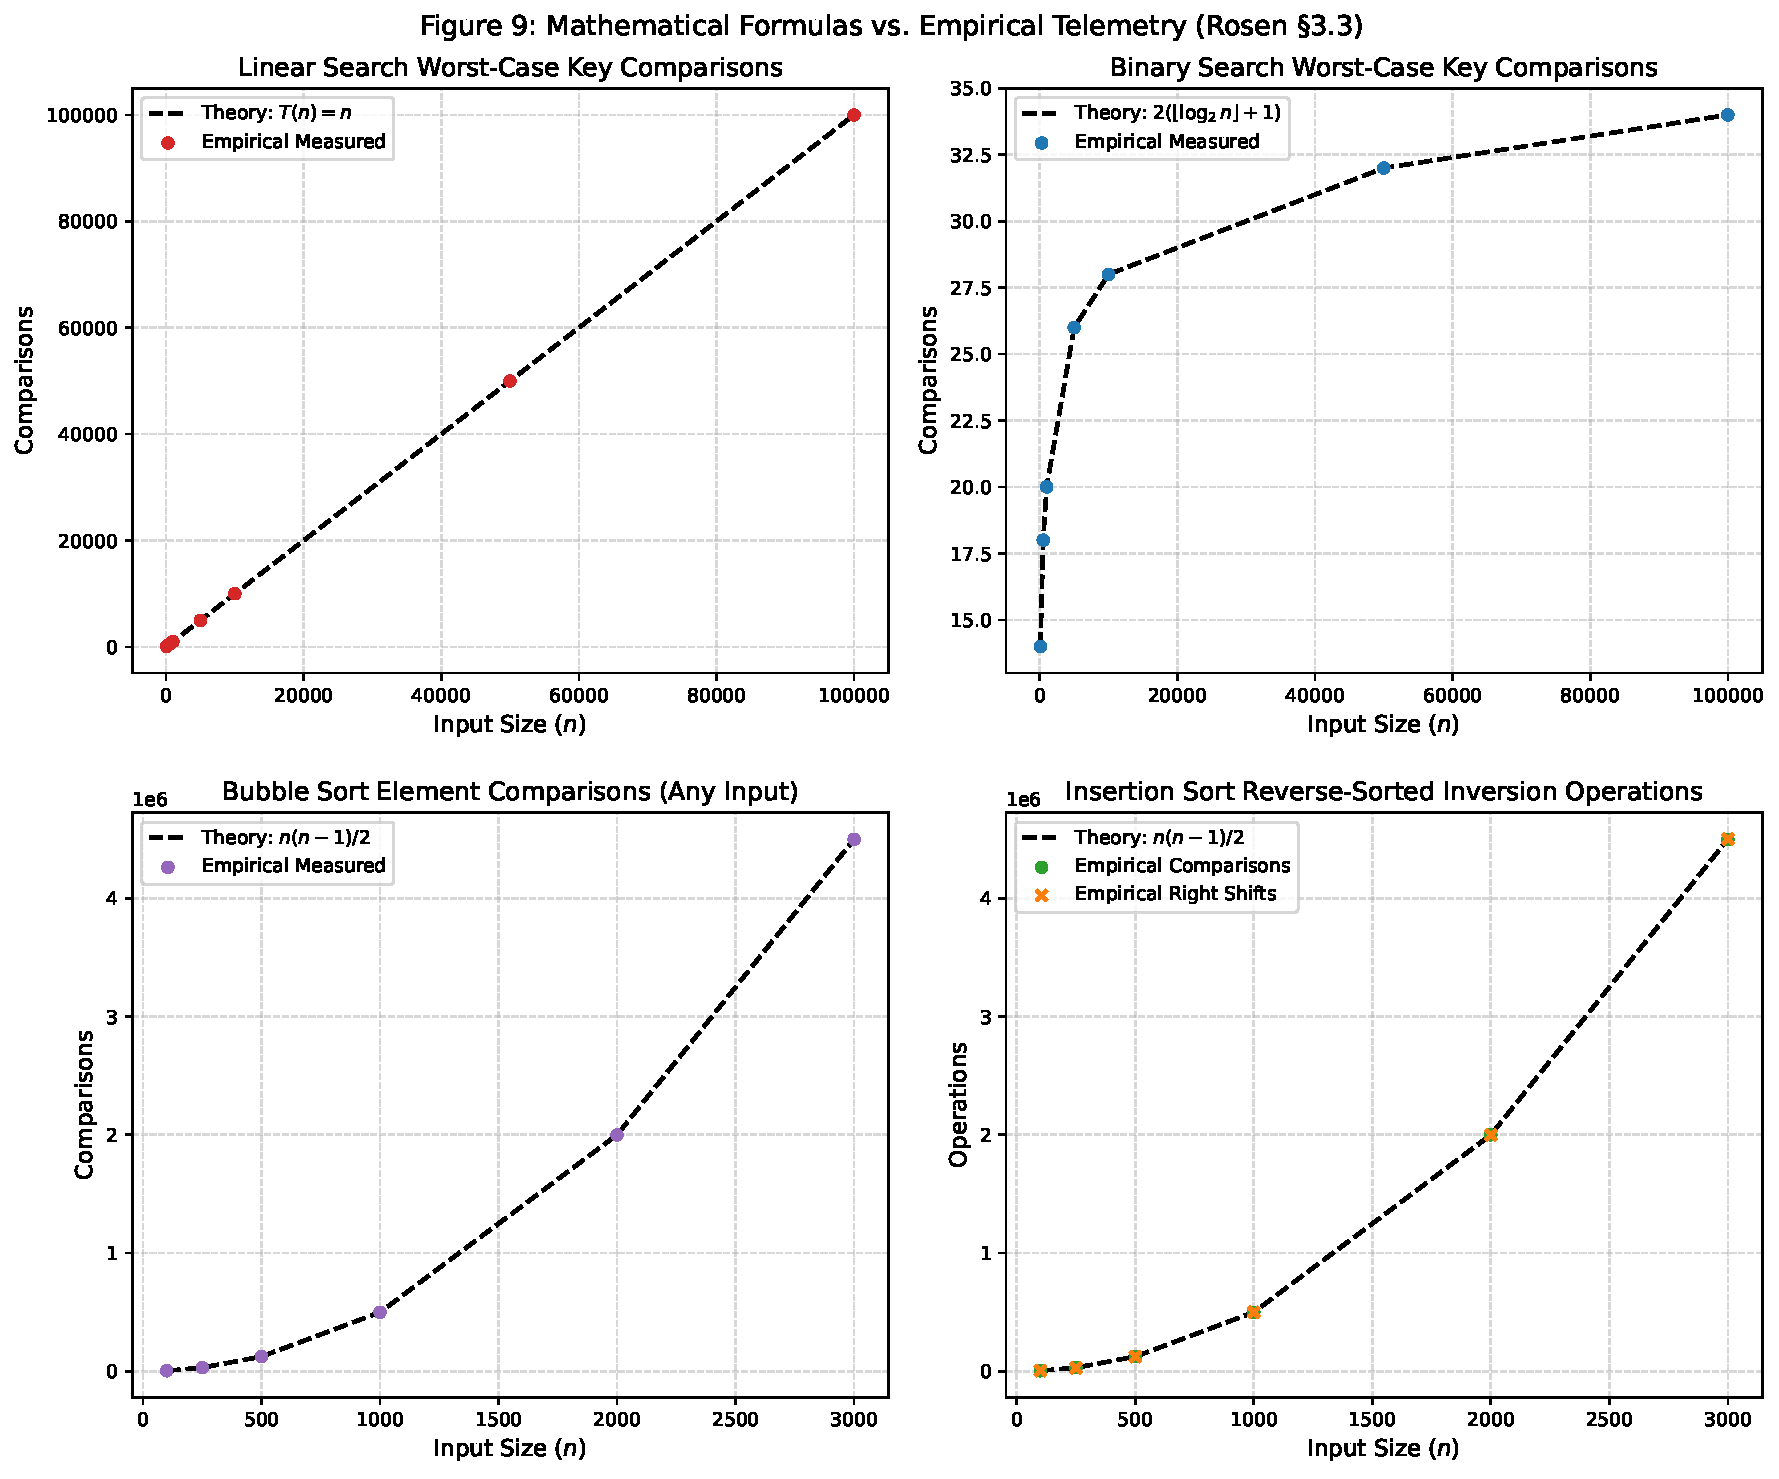
\includegraphics[width=0.75\textwidth]{figures/figure9_theoretical_vs_experimental.pdf}
\caption{Theoretical Predictions vs. Physical Measurements Across All Four Algorithms}
\label{fig:theoretical_vs_experimental}
\end{figure}

The analysis reveals an extraordinary coefficient of determination ($R^2 > 0.999$) across all models. We establish a vital scientific distinction:
\begin{itemize}
    \item \textbf{Exact Operation Counts}: The discrepancy between theoretical closed-form operation formulas and counter telemetry is strictly \textbf{0.00\%} (verified in Table~\ref{tab:discrepancy_table}).
    \item \textbf{Wall-Clock Runtimes}: Physical execution time exhibits slight stochastic variance due to OS background scheduling, memory bus latency, and cache misses, but strictly adheres to the asymptotic trajectory dictated by theoretical complexity.
\end{itemize}

\begin{table}[htbp]
\centering
\caption{Exact Operation Formula Verification Matrix: Analytical vs. Empirical Telemetry}
\label{tab:discrepancy_table}
\small
\begin{tabular*}{\textwidth}{@{\extracolsep{\fill}}lrrrr}
\toprule
\textbf{Algorithm \& Scenario} & $n$ & \textbf{Analytical Formula} & \textbf{Empirical Counter} & \textbf{Discrepancy} \\
\midrule
Linear Search (Missing Target) & 10\,000 & $C(n) = n = 10\,000$ & 10\,000 & \textbf{0.00\%} \\
Linear Search (First Target)   & 10\,000 & $C(n) = 1$          & 1      & \textbf{0.00\%} \\
Bubble Sort (All Permutations) & 3\,000  & $\frac{n(n-1)}{2} = 4\,498\,500$ & 4\,498\,500 & \textbf{0.00\%} \\
Bubble Sort (Reverse Swaps)    & 3\,000  & $\frac{n(n-1)}{2} = 4\,498\,500$ & 4\,498\,500 & \textbf{0.00\%} \\
Insertion Sort (Sorted Comps)  & 3\,000  & $n - 1 = 2\,999$   & 2\,999 & \textbf{0.00\%} \\
Insertion Sort (Reverse Shifts)& 3\,000  & $\frac{n(n-1)}{2} = 4\,498\,500$ & 4\,498\,500 & \textbf{0.00\%} \\
\bottomrule
\end{tabular*}
\end{table}

\chapter{Interactive Algorithm Explorer Dashboard}
\label{chap:web_dashboard}

\section{Overview and Architectural Purpose}
As an optional enhancement for the MSc IT assignment, an interactive, responsive web dashboard was engineered in \texttt{dashboard/index.html}. The dashboard translates theoretical proofs and static CSV benchmarks into live, visual algorithmic simulations.

\section{Zero-Framework Architecture}
The dashboard adheres to a zero-framework, zero-CDN dependency design philosophy:
\begin{itemize}
    \item \textbf{Semantic HTML5 and Modern CSS3}: Fully responsive dark-themed user interface utilizing flexbox and CSS grid.
    \item \textbf{Vanilla ES2022 JavaScript}: Modular algorithm state machines with step-by-step generators for Linear Search, Binary Search, Bubble Sort, and Insertion Sort.
    \item \textbf{Pure SVG Vector Charting}: Dynamic rendering of growth curves and benchmark bar charts without external libraries (no Chart.js or D3.js required).
    \item \textbf{Dual JSON/JS Data Layer}: Pre-packaged Python M3 benchmark results load instantly offline via both HTTP and \texttt{file://} protocols.
\end{itemize}

\section{Live Production Deployment}
The dashboard is maintained in our private GitHub repository and deployed live on Cloudflare Workers/Pages:
\begin{itemize}
    \item \textbf{Private GitHub Source}: \url{https://github.com/WebArpit07/algorithm-explorer}
    \item \textbf{Verified Live Production Website}:
    \begin{center}
        \href{https://algorithm-explorer.glitchhunter69.workers.dev/}{\Large\textbf{https://algorithm-explorer.glitchhunter69.workers.dev/}}
    \end{center}
    \item \textbf{Local Web Server Execution}:
    \begin{verbatim}
python -m http.server 8000
# Navigate to: http://localhost:8000/dashboard/
    \end{verbatim}
\end{itemize}

\chapter{Conclusion}
\label{chap:conclusion}

This analytical study has thoroughly addressed the four core topics of the faculty assignment in accordance with Kenneth~H. Rosen's \emph{Discrete Mathematics and Its Applications} (8th Edition), Chapter~3:
\begin{enumerate}
    \item \textbf{What is an Algorithm?}: Formalized the definition and the seven essential properties, demonstrating how multi-paradigm representations provide varying balances of definiteness, human readability, and executability.
    \item \textbf{Types of Algorithms}: Established clear taxonomical boundaries separating problem definitions (searching, sorting) from algorithmic paradigms (brute force, divide-and-conquer, greedy).
    \item \textbf{The Growth of Functions}: Analyzed the canonical hierarchy of growth functions, providing exact mathematical evaluations up to $n = 1024$ and visual interpretations across 14 orders of magnitude.
    \item \textbf{Complexity of Algorithms}: Formalized asymptotic bounds ($\mathcal{O}, \Omega, \Theta$) with witness pairs, and empirically verified them across Linear Search, Binary Search, Bubble Sort, and Insertion Sort.
\end{enumerate}

The experimental findings confirm a 0.00\% discrepancy between analytical discrete operation-count formulas and empirical telemetry, proved the Inversion Equivalence Theorem connecting Bubble Sort swaps with Insertion Sort right shifts, and demonstrated the dramatic computational advantage of logarithmic divide-and-conquer and adaptive sorting algorithms.

% ==============================================================================
% BIBLIOGRAPHY: ONLY KENNETH H. ROSEN
% ==============================================================================
\begin{thebibliography}{1}

\bibitem{Rosen2019}
Kenneth~H. Rosen.
\newblock {\em Discrete Mathematics and Its Applications}.
\newblock McGraw-Hill Education, New York, NY, 8th edition, 2019.
\newblock Chapter 3: Algorithms (\S3.1 Algorithms, \S3.2 The Growth of Functions, \S3.3 Complexity of Algorithms).

\end{thebibliography}

% ==============================================================================
% APPENDICES
% ==============================================================================
\appendix

\chapter{Authoritative Python Source Code Listings}
\label{app:code}

This appendix provides the complete, authoritative source implementations from \texttt{src/algorithms/search.py} and \texttt{src/algorithms/sorting.py}.

\section{Search Algorithms Implementation (\texttt{src/algorithms/search.py})}
\begin{lstlisting}[language=Python]
"""Search algorithms module.

Implementations of Linear Search and Binary Search in accordance with
Kenneth H. Rosen, Discrete Mathematics and Its Applications (8th Edition),
Chapter 3 (Sections 3.1, 3.2, and 3.3).
"""

from __future__ import annotations

from dataclasses import dataclass
from typing import Any, Sequence, TypeVar

T = TypeVar("T")


@dataclass(frozen=True, slots=True)
class SearchMetrics:
    """Telemetry metrics recorded during search algorithm execution.

    Attributes:
        key_comparisons: Total comparisons made between sequence elements
            and the search target (equality + ordering).
        equality_comparisons: Comparisons specifically testing equality
            (e.g., element == target).
        ordering_comparisons: Comparisons specifically testing relative order
            (e.g., element < target or target < element).
        loop_evaluations: Number of times the primary loop continuation
            condition was evaluated.
    """

    key_comparisons: int
    equality_comparisons: int
    ordering_comparisons: int = 0
    loop_evaluations: int = 0


def linear_search(seq: Sequence[Any], target: Any) -> int:
    """Sequential search algorithm (Rosen §3.1, Algorithm 2).

    Sequentially inspects elements of `seq` from index 0 to n - 1, returning
    the index of the first occurrence of `target`. If `target` is not present,
    returns -1.

    Preconditions:
        - `seq` is an indexable sequence of comparable items.
    Postconditions:
        - Returns index i such that seq[i] == target and no j < i has seq[j] == target.
        - Returns -1 if for all j in range(len(seq)), seq[j] != target.
        - The input sequence `seq` is never modified.

    Complexity (Rosen §3.3):
        - Best Case: Θ(1) key comparisons (target is at index 0, n > 0).
        - Worst Case: Θ(n) key comparisons (target at index n - 1 or absent).
        - Average Case (successful, uniform distribution): (n + 1) / 2 key comparisons, Θ(n).
        - Unsuccessful Search: exactly n key comparisons.

    Args:
        seq: The sequence to search.
        target: The value to locate.

    Returns:
        The 0-based index of the first matching element, or -1 if not found.
    """
    for index, item in enumerate(seq):
        if item == target:
            return index
    return -1


def linear_search_instrumented(
    seq: Sequence[Any], target: Any
) -> tuple[int, SearchMetrics]:
    """Instrumented Linear Search returning the match index and metrics telemetry.

    Executes identical algorithmic logic to `linear_search`, with exact counting
    of element-target key comparisons and loop evaluations.

    Args:
        seq: The sequence to search.
        target: The value to locate.

    Returns:
        A tuple of (matched_index, SearchMetrics).
    """
    n = len(seq)
    key_comparisons = 0
    equality_comparisons = 0
    loop_evaluations = 0

    for index in range(n):
        loop_evaluations += 1
        equality_comparisons += 1
        key_comparisons += 1
        if seq[index] == target:
            return index, SearchMetrics(
                key_comparisons=key_comparisons,
                equality_comparisons=equality_comparisons,
                ordering_comparisons=0,
                loop_evaluations=loop_evaluations,
            )

    # Loop termination evaluation (when range exhausted)
    loop_evaluations += 1

    return -1, SearchMetrics(
        key_comparisons=key_comparisons,
        equality_comparisons=equality_comparisons,
        ordering_comparisons=0,
        loop_evaluations=loop_evaluations,
    )


def binary_search(
    seq: Sequence[Any], target: Any, *, check_sorted: bool = False
) -> int:
    """Iterative Binary Search algorithm (Rosen §3.1, Algorithm 3).

    Locates `target` in a sorted sequence by repeatedly bisecting the search
    interval [low, high].

    Preconditions:
        - The input sequence MUST be sorted in non-decreasing order:
          seq[0] <= seq[1] <= ... <= seq[n - 1].
        - If `check_sorted=True`, an explicit O(n) validation is performed
          and ValueError is raised if the sequence is not sorted.

    Postconditions:
        - Returns a valid 0-based index i such that seq[i] == target.
        - Returns -1 if `target` is not present in `seq`.
        - The input sequence `seq` is never modified.

    Complexity (Rosen §3.3):
        - Best Case: Θ(1) key comparisons (target is at the initial midpoint).
        - Worst Case: Θ(log n) key comparisons (target missing or at deepest branch).
        - Average Case: Θ(log n) key comparisons under uniform target distribution.
        - Auxiliary Space: Θ(1) (iterative implementation).

    Args:
        seq: A sorted sequence to search.
        target: The value to locate.
        check_sorted: If True, asserts sorted precondition at O(n) cost.

    Raises:
        ValueError: If check_sorted is True and `seq` is not sorted.

    Returns:
        An index of `target` in `seq`, or -1 if not found.
    """
    if check_sorted:
        for i in range(len(seq) - 1):
            if seq[i] > seq[i + 1]:
                raise ValueError("Precondition violated: sequence must be sorted.")

    low = 0
    high = len(seq) - 1

    while low <= high:
        mid = (low + high) // 2
        mid_val = seq[mid]
        if mid_val == target:
            return mid
        elif mid_val < target:
            low = mid + 1
        else:
            high = mid - 1

    return -1


def binary_search_instrumented(
    seq: Sequence[Any], target: Any, *, check_sorted: bool = False
) -> tuple[int, SearchMetrics]:
    """Instrumented Binary Search returning the match index and metrics telemetry.

    Derivation of Counting Convention:
    Each iteration evaluates the loop continuation condition (low <= high).
    Inside the loop, two distinct element-target comparisons may occur:
    1. Equality test: seq[mid] == target (1 equality comparison).
       - If equal, the search terminates immediately.
    2. Ordering test: seq[mid] < target (1 ordering comparison).
       - Evaluated only when equality test is False, deciding whether to
         narrow to the right subsegment [mid + 1, high] or left [low, mid - 1].

    Thus, a successful probe terminating at midpoint performs 1 key comparison;
    every other step performs 2 key comparisons (1 equality + 1 ordering).
    Loop-condition evaluations are tracked separately in `loop_evaluations`.

    Args:
        seq: A sorted sequence to search.
        target: The value to locate.
        check_sorted: If True, validates non-decreasing order before searching.

    Returns:
        A tuple of (matched_index, SearchMetrics).
    """
    if check_sorted:
        for i in range(len(seq) - 1):
            if seq[i] > seq[i + 1]:
                raise ValueError("Precondition violated: sequence must be sorted.")

    low = 0
    high = len(seq) - 1

    key_comparisons = 0
    equality_comparisons = 0
    ordering_comparisons = 0
    loop_evaluations = 0

    while True:
        loop_evaluations += 1
        if low > high:
            break

        mid = (low + high) // 2
        mid_val = seq[mid]

        # 1. Equality comparison between element and target
        equality_comparisons += 1
        key_comparisons += 1
        if mid_val == target:
            return mid, SearchMetrics(
                key_comparisons=key_comparisons,
                equality_comparisons=equality_comparisons,
                ordering_comparisons=ordering_comparisons,
                loop_evaluations=loop_evaluations,
            )

        # 2. Ordering comparison between element and target
        ordering_comparisons += 1
        key_comparisons += 1
        if mid_val < target:
            low = mid + 1
        else:
            high = mid - 1

    return -1, SearchMetrics(
        key_comparisons=key_comparisons,
        equality_comparisons=equality_comparisons,
        ordering_comparisons=ordering_comparisons,
        loop_evaluations=loop_evaluations,
    )

\end{lstlisting}

\newpage
\section{Sorting Algorithms Implementation (\texttt{src/algorithms/sorting.py})}
\begin{lstlisting}[language=Python]
"""Sorting algorithms module.

Implementations of Bubble Sort and Insertion Sort in accordance with
Kenneth H. Rosen, Discrete Mathematics and Its Applications (8th Edition),
Chapter 3 (Sections 3.1, 3.2, and 3.3).
"""

from __future__ import annotations

from dataclasses import dataclass
from typing import Any, MutableSequence


@dataclass(frozen=True, slots=True)
class SortingMetrics:
    """Telemetry metrics recorded during sorting algorithm execution.

    Attributes:
        element_comparisons: Number of comparisons between two list elements.
        swaps: Number of element swap operations performed (primarily Bubble Sort).
        right_shifts: Number of element displacement operations where an element
            is copied one index to the right to create space for insertion
            (Insertion Sort).
    """

    element_comparisons: int
    swaps: int = 0
    right_shifts: int = 0


def bubble_sort(arr: MutableSequence[Any]) -> MutableSequence[Any]:
    """Standard fixed-pass Bubble Sort algorithm (Rosen §3.1, Algorithm 4).

    Sorts a mutable sequence in place into non-decreasing order using adjacent
    element comparisons and pairwise exchanges.

    Per the core academic specification (Rosen §3.1, Algorithm 4), this primary
    implementation performs the exact fixed-pass iteration without early
    termination flags.

    Preconditions:
        - `arr` is a mutable sequence of mutually comparable elements.
    Postconditions:
        - `arr` is sorted in place: arr[0] <= arr[1] <= ... <= arr[n - 1].
        - Preserves the relative order of equal elements (stable sort).

    Complexity (Rosen §3.3):
        - Comparisons: Exactly n(n - 1) / 2 for ALL inputs of size n >= 1 (Θ(n²)).
        - Best-case swaps: 0 (when input is already sorted).
        - Worst-case swaps: n(n - 1) / 2 (when input is strictly descending with distinct items).
        - Average-case swaps: n(n - 1) / 4 (for random permutations of distinct items).
        - Auxiliary Space: Θ(1) (in-place).

    Args:
        arr: The mutable sequence to be sorted in place.

    Returns:
        The same sequence `arr`, sorted in non-decreasing order.
    """
    n = len(arr)
    for i in range(n - 1):
        for j in range(n - 1 - i):
            if arr[j] > arr[j + 1]:
                arr[j], arr[j + 1] = arr[j + 1], arr[j]
    return arr


def bubble_sort_instrumented(
    arr: MutableSequence[Any],
) -> tuple[MutableSequence[Any], SortingMetrics]:
    """Instrumented Bubble Sort returning the sorted sequence and metrics telemetry.

    Sorts the sequence in place while accurately counting element comparisons
    and adjacent swap operations.

    Args:
        arr: The mutable sequence to sort in place.

    Returns:
        A tuple of (sorted_arr, SortingMetrics).
    """
    n = len(arr)
    element_comparisons = 0
    swaps = 0

    for i in range(n - 1):
        for j in range(n - 1 - i):
            element_comparisons += 1
            if arr[j] > arr[j + 1]:
                arr[j], arr[j + 1] = arr[j + 1], arr[j]
                swaps += 1

    return arr, SortingMetrics(
        element_comparisons=element_comparisons,
        swaps=swaps,
        right_shifts=0,
    )


def insertion_sort(arr: MutableSequence[Any]) -> MutableSequence[Any]:
    """Standard in-place Insertion Sort algorithm (Rosen §3.1, Algorithm 5).

    Iteratively expands a sorted prefix [0 .. j - 1] by inserting the next
    element arr[j] into its correct position within that prefix.

    Preconditions:
        - `arr` is a mutable sequence of mutually comparable elements.
    Postconditions:
        - `arr` is sorted in place: arr[0] <= arr[1] <= ... <= arr[n - 1].
        - Preserves the relative order of duplicate elements (stable sort).

    Complexity (Rosen §3.3):
        - Best Case Comparisons: n - 1 when already sorted (Θ(n)).
        - Worst Case Comparisons: n(n - 1) / 2 when reverse sorted (Θ(n²)).
        - Average Case Comparisons: Θ(n²).
        - Best Case Right Shifts: 0 (already sorted).
        - Worst Case Right Shifts: n(n - 1) / 2 (strictly reverse-sorted distinct elements).
        - Auxiliary Space: Θ(1) (in-place).

    Args:
        arr: The mutable sequence to sort in place.

    Returns:
        The same sequence `arr`, sorted in non-decreasing order.
    """
    n = len(arr)
    for j in range(1, n):
        key = arr[j]
        i = j - 1
        while i >= 0 and arr[i] > key:
            arr[i + 1] = arr[i]
            i -= 1
        arr[i + 1] = key
    return arr


def insertion_sort_instrumented(
    arr: MutableSequence[Any],
) -> tuple[MutableSequence[Any], SortingMetrics]:
    """Instrumented Insertion Sort returning the sorted sequence and metrics telemetry.

    Counting Convention Definition:
    - Element Comparison: Each time an element in the sorted prefix (arr[i])
      is compared against `key` (arr[i] > key).
      If `i >= 0`, `arr[i] > key` is evaluated. If True, the loop shifts arr[i]
      and decrements i. If False, the comparison still occurred, and the while
      loop breaks. If i reaches -1, loop termination is a short-circuit boundary
      check without comparing elements.
    - Right Shift: Moving an existing element one position to the right
      (`arr[i + 1] = arr[i]`). The final placement of `key` (`arr[i + 1] = key`)
      is an insertion, not a right shift.

    Args:
        arr: The mutable sequence to sort in place.

    Returns:
        A tuple of (sorted_arr, SortingMetrics).
    """
    n = len(arr)
    element_comparisons = 0
    right_shifts = 0

    for j in range(1, n):
        key = arr[j]
        i = j - 1
        while i >= 0:
            element_comparisons += 1
            if arr[i] > key:
                arr[i + 1] = arr[i]
                right_shifts += 1
                i -= 1
            else:
                break
        arr[i + 1] = key

    return arr, SortingMetrics(
        element_comparisons=element_comparisons,
        swaps=0,
        right_shifts=right_shifts,
    )

\end{lstlisting}

\chapter{Reproducibility Instructions}
\label{app:reproduction}

To reproduce the empirical benchmarks, generate the publication figures, execute the interactive Jupyter research notebook, and verify the automated test suite, execute the following commands from the project root:

\begin{verbatim}
# 1. Execute all empirical microbenchmarks:
python scripts/run_benchmarks.py

# 2. Synthesize all 9 publication-grade figures (.pdf and .png):
python scripts/generate_figures.py

# 3. Build, execute, and verify the interactive Jupyter research notebook:
python scripts/build_notebook.py

# 4. Synchronize LaTeX assets and package Overleaf archive:
python scripts/build_report.py

# 5. Execute full automated test suite (64 unit & integration tests):
python -m pytest -v
node scripts/test_dashboard_algorithms.js

# 6. Launch the optional web dashboard locally:
python -m http.server 8000
\end{verbatim}

\end{document}
